\documentclass[12pt]{report}
\usepackage[english]{babel}
\usepackage[utf8x]{inputenc}
\usepackage{hyperref}
 \hypersetup{colorlinks = true}
\usepackage{amsmath}
\usepackage{amssymb}
\usepackage{graphicx}
\usepackage{multirow}\usepackage{multirow}
\usepackage{booktabs}
\usepackage{array}
\usepackage{verbatim}
\usepackage{textcomp}
\usepackage{lmodern}
\usepackage{blindtext}
\usepackage{apacite}
\usepackage{setspace}
\usepackage{titlesec}
\usepackage{longtable}
\usepackage{lscape}
\usepackage{float}
\usepackage{pdflscape}
\usepackage{tabu}
\usepackage[parfill]{parskip}
\usepackage{indentfirst}
\usepackage{adjustbox}
\usepackage[a4paper,top=1.0cm,bottom=1.5cm,left=2.5cm,inner=2.0cm,outer=2.0cm,bindingoffset=.5cm]{geometry}
\usepackage[colorinlistoftodos]{todonotes}
\usepackage{caption}
\usepackage{listings}
\usepackage{textgreek}
\usepackage[flushleft]{threeparttable}
\usepackage{rotating}
\usepackage{placeins}
\usepackage{blindtext}
\usepackage{multirow}
\usepackage{booktabs}
\usepackage{pdfpages}
\usepackage{tabularx}
\onehalfspace
\renewcommand{\arraystretch}{1.2}   
\newcommand\MyHead[2]{%
  \multicolumn{1}{l}{\parbox{#1}{\centering #2}}
}
\title{Access to primary health care and ambulatory care sensitive hospitalisations in the Maldives}
\author{Fazeela Mohamed \\ Student ID: 84483359 \\}
\begin{document}
\maketitle
\tableofcontents
\newpage
%%%%%%%%%%%%%%%%%%%%
%Done - send in word document
% Please do not remove the instructions or comments!
% If you want to indicate that you have worked on the 
% comments, write "done";if you do not want to work on 
% the comments, briefly mention the reason why you would not work on 
% the comments; if you want to work on the comments later,
% write "to do" or something similar to indicate that you
% will work on the comments later.
% You need to write a summary, ideally a one page summary
% of the proposal (title it: "Executive summary")
% In the summary, include the following: 
% (1) the problem you are investigating or a brief 
% introduction and background (about 1/3 rd of the page)
% (2) a short paragraph stating the goal, objectives, and main hypotheses
% (3) a summary of the methods
% (4) Significance of the work
% The potential examiners of your thesis proposal will be
% sent the proposal first; on their acceptance, we will 
% forward the full proposal
%%%%%%%%%

%Done- change the last segment ("and assess the extent to which those with ambulatory care sensitive conditions (ACSCs) - hypertension, chronic heart disease, diabetes, asthma, and chronic obstructive pulmonary disease have access to PHC") to reflect the second item "To assess the association between self-reported access to PHC services in the Maldives and risk of ACSH." in the objectives. So it should read something like, "assess the association between access to primary health care and risk of ambulatory care sensitive hospitalisation" 
%removed as per Arin's comment in drop box document "Likelihood of ACSH are high among those with ACSCs with low levels of self-reported access compared to general healthy population".

\chapter{Introduction}

The Maldives health care system is based on a primary health care (PHC) model. One of the health sector top priorities in the health master plan of the Maldives is to increase access to PHC services for all residents \cite{MOH:health:plan}. The health master plan outlines the national health goals and public health priorities. Measuring access to PHC in the Maldives is essential for achieving the desired health outcomes of decreasing the occurrence of avoidable hospitalisations and increasing the efficient use of health care resources \cite{MOH:health:plan}. 

Since the Maldives is a country with a challenging health care delivery system due to spatial characteristics of the islands and population, access to health care services are limited \cite{MOH:health:plan}. The health care delivery system has a unique setup that caters for the needs of the population. The public health care sector contributes to the majority of health care services in the Maldives. It is achieved through a three-tier system of health care delivery \cite{MOH:health:plan}. The referral system flows from primary through to secondary and tertiary -Figure~\ref{MHS}. Limited PHC facilities are available in every inhabited island. PHC is delivered from all hospital levels. Island health care centres are at PHC level. Secondary health care facilities in few selected islands are in two different levels: level 1 - atoll hospitals and level 2 - regional hospitals. Tertiary health care facilities are only available in the capital city Male'. Each inhabited island has one single island health centre that provides PHC. PHC for the islanders with atoll or regional hospitals are provided by atoll and regional hospitals. PHC for residents of Male' are provided by primary health centre named 'Dhamana Veshi' and tertiary healthcare facilities. This is provided by both public and private healthcare facilities. Private health care is mainly accessible from the capital city Male'.

In the Maldives, PHC services are available on walk-in basis. No appointments are required to see a general physician (GP). People of the Maldives do not have a specific regular GP. Any GP available at the outpatients department will attend to the patients in queue order. Therefore, there are long waiting times in accessing PHC services which are more evident in the capital city Male'. Since private healthcare is financed by means of out-of pocket, private insurance, and is subsidised by publicly funded scheme to some extent, not every resident can afford private health care services to bypass the long waiting time leading to disparities in access to healthcare services. 
 
The rural dwellers are disadvantaged in comparison to urban counterparts in access to health care services in the Maldives. The inhabitants of small, remote, and isolated islands are subjected to travel between islands as a result of limited PHC services in smaller islands \cite{MOH:health:plan}. This is due to shortage of skilled health care workers, inconsistent supply of medications, and impaired management of island health care centres \cite{MOH:health:plan}. It has weakened the trust in PHC services \cite{health:profile:2010}. 

To seek PHC, rural residents may have to travel from one level to other -Figure~\ref{map}. For example; If care is not available from island health centre, rural residents may have to travel to atoll hospital, regional hospital, and finally to tertiary health facilities in Male' depending on the availability of services. However, these rural residents often find it difficult to contact different levels of healthcare facilities as a result of impaired transportation services \cite{MOH:health:plan}. For rural residents, the cost of seeking healthcare services include cost of transport, and travel time between islands by sea boats. In cases of emergency, patient transfer is covered by universal health coverage - 'Asandha'. 

\begin{figure}[H]
\caption{Travel from one level to other}
\label{map}
\centering
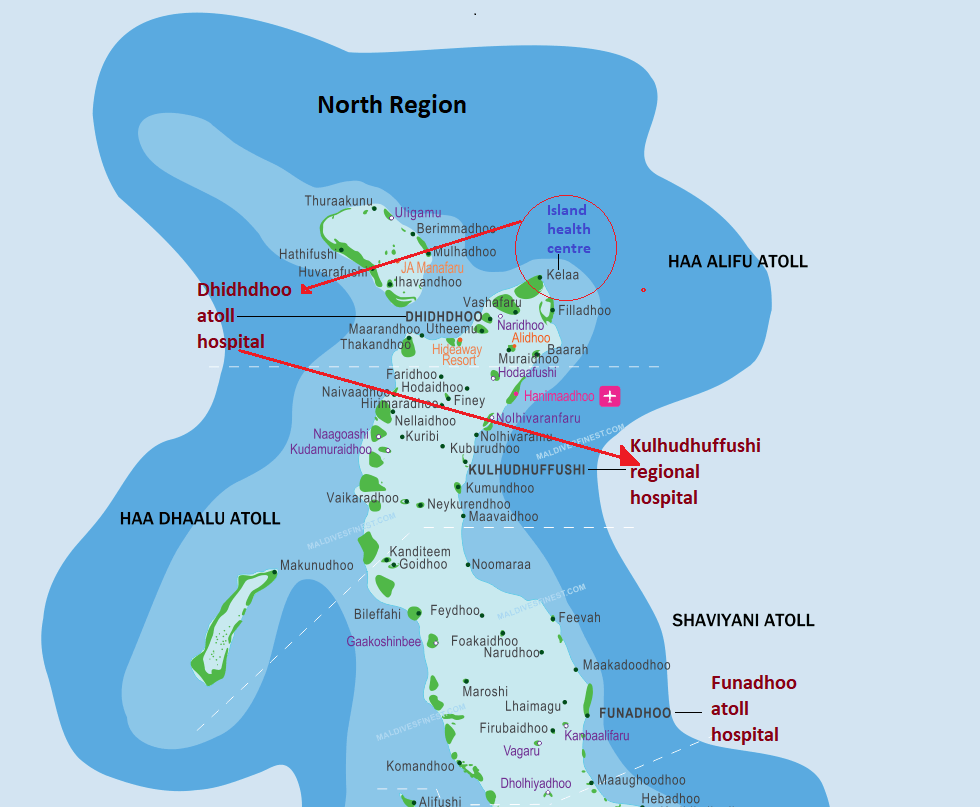
\includegraphics[width=1.0\textwidth]{northmap.png}
\end{figure}


\begin{figure}[H]
\caption{The Maldives health care system}
\label{MHS}
\centering
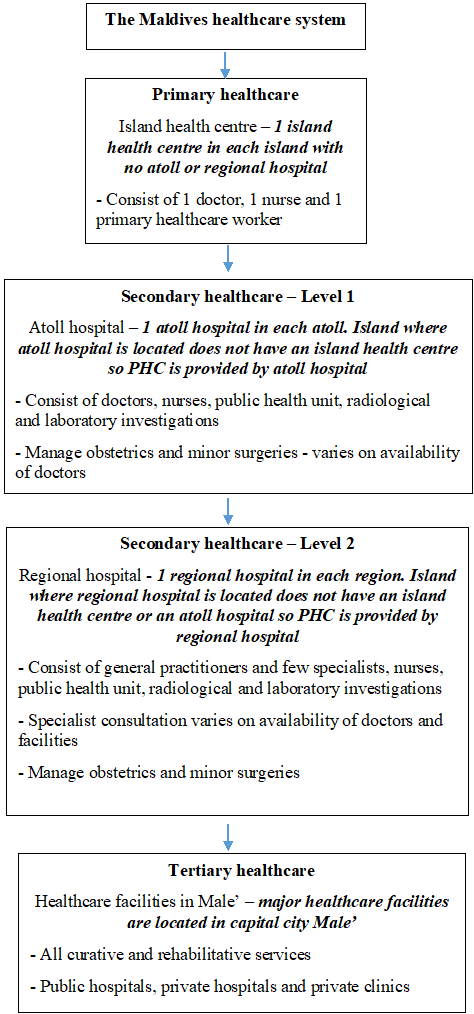
\includegraphics[width=0.70\textwidth]{MaldivesHS.png}
\end{figure}

\section{Ambulatory care sensitive hospitalisations} 

Ambulatory care sensitive hospitalisations (ACSH) is used as a proxy to indicate a failure or inadequacy of access to PHC services. ACSH is a set of preventable or avoidable hospitalisations where the setting of avoidance is in the PHC that are considered to be delivered in ambulatory setting \cite{barker2016pathways}. An ambulatory setting is a PHC setting where the patient is mobile, unlike hospitalised or institutionalised care setting where the patient is tethered to a bed for care to be provided.
 \cite{WHO:assess:acsh, magan2011hospitalizations,billings1990uninsured}.  
 
Ambulatory care sensitive conditions (ACSCs) are disease conditions where preventive care is delivered through outpatient departments or in the community which reduces hospitalisation due to their consequences \cite{ansari2012patient,ansari2002victorian,millman1993access}.  These conditions include asthma, diabetes, chronic heart failure (CHF), chronic obstructive pulmonary disease (COPD), and hypertension. Failure to have access to PHC can lead to chronic exacerbation of ACSCs, which can ultimately lead to hospitalisation \cite{ansari2012patient,ansari2002victorian,millman1993access}.

\section{Primary health care}

Equity and access to basic healthcare services was declared as rudimentary human right by declaration of Alma-Ata in 1978 \cite{Alma:ata:declaration}. The Declaration of Alma-Ata \citeyear{Alma:ata:declaration} expressed the need to protect and promote health of all people around the world. The declaration adopted PHC as a means of proving a comprehensive, cost-effective, equitable and universal health care service for populations around the world. Thereby, defining PHC as "essential health care based on practical, scientifically sound and socially acceptable methods and technology made universally accessible to individuals  and families in the community through their full participation and at a cost that the community and country can afford to maintain at every stage of their development in the spirit of self-reliance and self-determination. It forms an integral part both of the country's health system, of which it is the central function and main focus, and of the overall social and economic development of the community. It is the first level of contact of individuals, the family and community with the national health system bringing health care as close as possible to where people live and work, and constitutes the first element of a continuing health care process" \cite{Alma:ata:declaration}. In 2018, 120 countries renewed their commitment to PHC with Astana declaration \cite{walraven20192018}. Astana declaration aims to refocus on PHC \cite{Astana:PHC:action}.

PHC is envisaged to provide basic health care services on education and promotion of health and well-being; prevention and control of diseases; appropriate treatment and provision of essential drugs; and systematically addressing determinants of health \cite{vision:PHC:21century}. According to WHO \cite{vision:PHC:21century} the attainment and sustainability of universal health coverage and health related sustainable development goals can only be achieved with stronger emphasis on PHC. PHC has changed the emphasis from larger tertiary hospitals that are mostly available in urban areas to a more community-based delivery services with an inter-sectoral approach  \cite{to2003health}. Inter-sectoral approach is a multi-institutional collaboration to provide comprehensive and accessible health care services for the populations \cite{Inter:sectoral:action}. The actions of these institutions affect the health outcomes of the populations \cite{Inter:sectoral:action}. 

\section{Ambulatory care sensitive hospitalisations and primary health care}

Theoretically, in any health system that has high rates of ACSH, it can be argued that either people in that system have low levels of PHC services access and usage, or that the system fails to meet the needs of people to provide these services or both \cite{ansari2012patient,ansari2006access,laditka2003hospital,bindman1995preventable,billings1993impact,millman1993access}. In any case, patients have low levels of access to PHC in the community. Findings from research by Ansari and colleagues suggests that access was associated with rates of ACSH $(R^2=0.29;p=0.001)$ \cite{ansari2006access}. The estimated co-efficient -20.64 of this study suggests that every increment in level of access to PHC, reduces the rate of ACSH by 20.64 per 1000 persons. Edes and others supported this with their study in 31 European countries \cite{edes2014better}. Countries with better access to PHC were associated with lower rates of hospitalisation for patients with diabetes suggesting that every increment in level of access, reduced the rates of ACSH by 0.40 per 100,000 population \cite{edes2014better}. In California Bindman and colleagues found that reported poor access to PHC for ACSCs such as asthma, hypertension, CHF, COPD and diabetes between the ages 15-64 was inversely associated with higher rates of hospitalisations - $R^2=0.50;p<0.001$ \cite{bindman1995preventable}.

ACSH rates have been reported to be lower in health systems with a stronger primary health sector in different countries \cite{rosano2012relationship}. PHC increases access to health services and stronger PHC has shown to reduce ACSH contributing to an overall of 5\% in Brazil \cite{macinko2011influence}. More specifically, hospitalisation for cardiovascular diseases, asthma, hypertension, and stroke declined by 25 to 30\% with better PHC and access to these services \cite{macinko2010major}.  Research findings by Souza showed 82.3\% reduction in hospitalisation for asthma following PHC intervention program for control of asthma in Bahia between 1998 to 2006 in Salvador city \cite{souza2010rapid}. A negative correlation was found between the provision of basic asthma medication and hospitalisation (-0.801 / $p<0.0001$). Findings of research suggest that better PHC and access to these services were associated with lower hospitalisation rates for patients with diabetes - p=0.023, 95\%CI 0.9979-0.9998 \cite{calderon2014does}. Kravet and others found that an overall 15\% of increase in PHC decreased an estimated in-patient admissions by 6\%, emergency room visits by 10\%, and surgeries by 7\% \cite{kravet2008health}.

\section{Global phenomenon of ambulatory care sensitive conditions and primary health care}

The prevalence of ACSCs is more than 1 billion in 2017 \cite{GHD:health:2017}. Amongst this cardiovascular diseases including hypertension, CHF, and other heart diseases accounts for more than 485 million in the same year. According to WHO reports, 17.9 million people die each year from cardiovascular diseases which is an estimated 31\% of the total deaths world wide \cite{WHO:health:2018}. Eighty five percent (85\%) of the cardiovascular deaths are due to heart attacks and strokes \cite{WHO:health:2018}. Seventy five percent (75\%) of these deaths occur in low and middle income countries such as the Maldives \cite{WHO:health:2018}. 
Hypertension which WHO describes as the "silent killer" of 21st century is one of the major contributors to deaths. In this regard, 40\% of the adults above 25 years of age are estimated to have raised blood pressure which is considered to be every 1 in 3 adults worldwide \cite{WHO:health:2018}. In South-East Asia, 36\% adults above 25 years are estimated to have hypertension \cite{WHO:health:2018}. The prevalence of high blood pressure is higher among low-middle and upper-middle income countries accounting for 40\%. Nearly nine and a half million people die every year due to complications related to hypertension \cite{WHO:health:2013}. In 2013, WHO report highlights health and economic costs associated with inadequate treatment and poor control of hypertension at PHC level, such as expensive interventions like bypass surgery and dialysis; and premature mortality due to stroke and heart diseases which can drain individuals and governments' budget \cite{WHO:health:2013}. It could also lead to poor health status, disability or premature mortality. It is suggested that proper access to PHC through early detection, treatment, and management of hypertension will help to avoid associated complications leading to a better health status and avoidance of unnecessary economic burden \cite{WHO:health:2013}.  

CHF is considered as an epidemic that reflects the increase incidence of this condition every year \cite{roger2013epidemiology}. The prevalence of CHF constitutes for more than 23 million world wide \cite{roger2013epidemiology}. Roger suggests that "progress in primary prevention of CHF would lead to decreasing incidence of disease while improvement in medical care would improve the survival" \cite{roger2013epidemiology} p.2. PHC plays a major role in reducing the burden of hospitalisation due to complications among patients living with CHF. If CHF is not managed at the PHC setting the survival estimates are 50\% which reduces to 10\% in ages 5 to 10 years \cite{chugh2008epidemiology,cowie2000survival}. It can also increase the risk of sudden death \cite{chugh2008epidemiology}.

According to WHO, patients diagnosed with diabetes have reached 422 million in 2014 compared to 108 million in 1980 \cite{WHO:health:2018}. The global prevalence of diabetes among patients above 18 years of age has increased from 4.7\% in 1980 to 8.5\% in 2014 \cite{WHO:health:2018}. It is higher among the low and middle income countries such as the Maldives. It is estimated that 1.6 million deaths in 2016 were caused by diabetes and 2.2 million deaths from high blood glucose level \cite{WHO:health:2018}. WHO reports uncontrolled diabetes as one of the main reasons for blindness, kidney failure, heart attacks, stroke, and lower limb amputation \cite{WHO:diabetes:2016}. It was reported that during pregnancy, poorly managed diabetes can increase the risk of fetal death and other complications. The report further highlights that complications related to diabetes can lead to substantial economic loss for patients living with this condition, and their families in terms of medical costs, and lost of wages; and health care system such as resources. WHO suggests that proper access to PHC for patients with diabetes is essential to reduce the complications \cite{WHO:diabetes:2016}. 

Preventable chronic respiratory diseases such as asthma and COPD kills more than 4 million people every year \cite{WHO:asthmacopd:2007}. Over 400 million people live with these conditions in low and middle income countries \cite{WHO:asthmacopd:2007}. According to global burden of disease study, more than 251 million people are diagnosed with COPD in 2016 \cite{WHO:health:2018}. An estimated 3.7 million people died due to COPD in 2015 \cite{WHO:health:2018}. This corresponds to 5\% of total deaths globally. It is the third leading cause of death in the world. 90\% of these deaths occur in low to middle income countries such as the Maldives. COPD is estimated to increase in the years to come due to raise in prevalence of smoking and ageing populations globally. Management of disease at PHC setting and in community can help to relieve the symptoms, improve the quality of life of people with COPD, and reduce the risk of premature death \cite{WHO:health:2018}. This includes appropriate treatment and patient health education.

It is estimated that 235 million people around the world suffer from asthma \cite{WHO:health:2018}. In 2015, 383,000 deaths were caused by asthma \cite{WHO:health:2018}. Many of these deaths are as a result of lack of access to basic asthma medications and PHC \cite{WHO:asthmacopd:2007}. Less access to PHC can lead to poor quality of life for patients with this condition \cite{WHO:asthmacopd:2007}. It can cause considerable economic loss in-terms of use of hospital resources for complications due to poorly managed asthma. 

\section{Ambulatory care sensitive conditions in the Maldives}

In the Maldives, non-communicable disease constitutes 78\% of the total disease burden, in which cardiovascular diseases including hypertension and CHF, COPD, asthma, and diabetes are among the top 10 diseases \cite{Maldives:healthprofile:2016}. ACSCs are the leading causes of death in the Maldives \cite{WHO:country:strategy}. It contributes to 81\% of deaths \cite{WHO:country:strategy}. In  2017, in the Maldives, 37.2\% of premature death accounts for COPD, asthma, diabetes, hypertensive diseases, and cardiovascular diseases which is relatively high in comparison to 27\% globally in the same year \cite{GHD:health:2017}. Disability adjusted life years (DALY) amongst patients with ACSCs have continued to increase in the Maldives by 1.2\% annually which has reached 51.2\% in 2017 \cite{GHD:health:2017}. In the Maldives, 20\% of the population above 18 years of age are diagnosed with high blood pressure \cite{WHO:profile:country}. It is estimated that high blood pressure constitutes 12\% of the total deaths and DALY in the Maldives \cite{GHD:health:2017}. It is one of the leading causes of CHF and other heart diseases. About 9\% of the Maldivian population above 18 years of age are diagnosed with diabetes \cite{WHO:profile:country}, 16.9\% death and 4.36\% DALY also account for diabetes \cite{GHD:health:2017}. The prevalence of chronic respiratory diseases - asthma and COPD was 6.41\% in 2017 \cite{GHD:health:2017}. It is estimated that COPD accounts for 11.84\% of death and DALY in the Maldives  \cite{GHD:health:2017}. COPD accounts for 46\% of total deaths by respiratory diseases in 2016 which is 13\% increase from 2015 \cite{Maldives:nationalhealthstatistics:2019}.

\section{Ambulatory care sensitive hospitalisations in the Maldives, Singapore, New Zealand, and United Kingdom}

ACSH is a problem in the Maldives, similar to other island nations such as New Zealand, United Kingdom, and Singapore. This is not different in high income countries in comparison to the Maldives - a middle income country. Data from island nations Singapore, New Zealand, and United Kingdom for ACSH report that the figures have decreased in New Zealand from 26\% in 2012 to 24\% in 2014\cite{OECD:Data:countries}. It remained steady in the United Kingdom at 25\% over the same time period \cite{OECD:Data:countries}. Another island nation in Asia, Singapore has registered an increase in ACSH from 22\% in 2011 to 25\% in 2014 \cite{OECD:Data:countries}. Among the ACSCs, COPD accounts for highest percentage of hospitalisations in 2014 in New Zealand (48\%), and United Kingdom (48\%) in comparison to 18\% in Singapore \cite{OECD:Data:countries}. Hospitalisation for hypertension accounts for least percentage in this year for New Zealand 2\%, United Kingdom 3\% and Singapore 3\% \cite{OECD:Data:countries}. Hospitalisation for asthma remained relatively stable in New Zealand 9\% from 2012 to 2014 while in United Kingdom increased 13\% in 2013 to 15\% in 2014 in comparison to Singapore that decreased from 12\% in 2011 to 10\% in 2014 \cite{OECD:Data:countries}. Hospitalisation for CHF increased considerably at a higher rate in United Kingdom from 21\% in 2011 to 30\% in 2014 while it reduced in Singapore from 31\% in 2011 to 26\% in 2014 \cite{OECD:Data:countries}. Hospitalisation for diabetes remained static in United Kingdom (14\%) while in New Zealand decreased from 24\% in 2013 to 20\% 2014 \cite{OECD:Data:countries}. This is different to Singapore where hospitalisations for diabetes increased considerably from 28\% in 2011 to 43\% in 2014 \cite{OECD:Data:countries}. 

% Done - Do you have data from Japan and Iceland? If not, instead of writing "aggregated data from developed nations", change to data from ....(list of countries). Also, as you have not
% aggregated any data yourself, avoid "aggregated"
% *if time allows in to do list* - Iceland 

In comparison to Singapore, New Zealand, and United Kingdom, ACSH accounts for 36\% of total non-communicable hospitalisations in the Maldives \cite{Maldives:nationalhealthstatistics:2019}. These include 24\% cardiovascular diseases including hypertensive heart diseases, and cerebrovascular diseases; 10\% respiratory diseases including asthma and COPD; and 2\% diabetes. Hospitalisations for hypertensive heart diseases accounts for 10\%. Hospitalisation for COPD is relatively high that accounts for 40\% in comparison to asthma that is 16\% of total hospitalisations for respiratory diseases. 

\section{Impaired access to primary health care and ambulatory care sensitive hospitalisations}

Findings from research suggests that impaired access to PHC risk the chances of ACSH as consequences. A study by Khader and others found that 15 to 18\% of patients with hypertension who failed to access appropriate PHC services were found to be hospitalised for complications such as stroke \cite{khader2012cohort1}. If patients with hypertension were able to access PHC and be treated in the outpatients and in the community, then this would have reduced the risk of hospitalisation \cite{ansari2012patient,ansari2006access,laditka2003hospital,bindman1995preventable,billings1993impact,millman1993access}. Furthermore, research showed that 10 to 20\% of patients with diabetes who failed to access appropriate PHC services were found to be hospitalised for complications such as blindness, stroke, and amputations \cite{khader2012cohort}. Such data on admissions based diabetes lower extremity amputation in island nations, New Zealand and United Kingdom registered a total of 8.7\% in 2017 \cite{OECD:Data:countries}. If these patients in New Zealand, and United Kingdom were treated in a PHC setting and diabetes were controlled, then it may either eliminate the need for organ amputation altogether or at least, lead to a much delayed or avoided hospitalisation. 

It is argued that increase in ACSH can squander the health care resources which may be utilised for other priority areas \cite{basu2008systematic,culler1998factors} such as healthcare budget. \cite{bodenheimer2002improving}. Findings from Harrison and others suggest that an estimated 8\% reduction in ACSH equivalent to 53,000 emergency admissions across England has a potential cost saving of around 149 million dollars per year \cite{harrison2014effect}. Wagner and others found that controlled glycemic levels through PHC reduces the rates of ACSH among patients with diabetes, reducing a total healthcare cost of 685-950 dollar per patient annually in Washington state \cite{wagner2001effect}. A similar study on adult asthma by Bolton and colleagues suggested that access to proper PHC within a period of 12 months may reduce healthcare costs by 628 dollars per patient in the United States \cite{greineder1999randomized}.

\section{Risk of ambulatory care sensitive hospitalisations}

The risk of ACSH due to impaired access to PHC is as a result of a range of factors including contextual factors and individual characteristics. Contextual factors are those that are best described as characteristics of the community and health care provider associated with access to PHC. Such variables include availability of health insurance coverage, organisation of services, supply or provision of the set of services by health care providers, and accessibility to these services. Individual characteristics are those that are associated with access to PHC services and pertain to 'individuals'. Such variables include an individual's response to sickness and treatment, biological imperatives, socio-economic background, and individual's personal resources.

Spatial correlation to ACSH of different counties in United States is observed as nearly 1, indicating strong relationship with geographical differences in access to PHC services \cite{mobley2006spatial}. The 2001 United Sates household travel survey showed 31.4\% rural residents take longer travel time to access PHC \cite{probst2007effects}. Probst and others found that travel time and travel distance are statistically associated with access to care $p<0.0001$ \cite{probst2007effects}. 

Archury and colleagues found that transportation was associated with health care visits and respondents who had family or friends who could provide transportation had 1.58 times better utilisation of health care services than those who did not \cite{arcury2005effects}. Further, a systematic literature review of 61 studies showed that transportation is an important factor in access to health care services \cite{syed2013traveling}. It was found that transportation was linked with timely medical care and medication access. 

It is observed that lower availability of PHC is associated with higher ACSH \cite{Parchman1999preventable}. Medicare patients in United States, residing in PHC shortage area are 1.82 times more likely to experience a preventable hospitalisation $(X^2=7.42, p<0.01, 95\%CI:1.18-2.81)$ than other patients \cite{Parchman1999preventable}. Having regular source of care has shown to significantly reduce ACSH \cite{Falik2001ambulatory, Gill1998the}. Patients receiving regular outpatient care from Federally Qualified Health Centres in United States are 1.5\%, $p<0.007$ less likely to experience ACSH when compared to patients (1.9\%) who do not receive outpatient care from these health centres \cite{Falik2001ambulatory}. Discrete-time hazard models that estimate risk of ACSH indicate issues with access and quality of PHC are associated with physician supply, and physician practice behaviour \cite{laditka2004physician}. Adequate physician supply can significantly decrease the risk of ACSH by 43\% \cite{laditka2004physician}. Various other researchers have supported that access is positively associated with physician supply \cite{basu2002primary,laditka2005more, parchman1994primary}. Friedman and colleagues found  significantly higher rates of ACSH among uninsured and medicaid patients of United States accounting for 42\% in comparison to privately insured patients 13\% \cite{friedman2001health}. National hospital discharge survey 1980-1998 data shows ACSH increased from 5.1\% in 1980 to 11.6\% in 1998 among uninsured persons in United States \cite{kozak2001trends}.

Falik and colleagues found that ACSH differ among age groups \cite{Falik2001ambulatory}. It is higher among children younger than 15 years accounting for 1.9\% in comparison to adults 1.5\% among the Federally Qualified Health Centre patients in the USA. Among these patients, 14\% experienced more than one readmission for same or other ACSCs. Rural residence has a strong association with likelihood of ACSH for these patients. A similar study in North Carolina shows contrasting figures \cite{ricketts2001hospitalization}. ACSH among 65 years and above were twice as higher (19.0/1000) in comparison to patients below the age of 65 years (10.15/1000). North Carolina has a relatively even distribution of urban 45\% and rural 55\% population. ACSH is found to be moderately associated with type of residence (r=0.54) for North Carolina. A study on ACSH associated with race, and ethnicity in United States shows that ACSH differ among gender, race, and ethnicity \cite{laditka2003hospital}. Non-Hispanic white men 21.56\% and women 15.50\% had higher rates of ACSH than Hispanic men 18.75\% and women 12.08\% between ages 19 to 64 years. This is different compared to ages above 65 years. Hispanic women (52.87\%) had higher rates of ACSH than non-Hispanic white women (41.38\%). Same study shows that African American women are 60\% more likely to experience ACSH than non-Hispanic white women. 

A six-year descriptive analysis of ACSH among migrant refugees in Australia shows that ACSH are higher among migrants in a ratio of 1:0 than Australia born persons \cite{correa2007six}. Ansari and others found that individual's income, and education are associated with ACSH \cite{ansari2006access}. The rates of ACSH are positively associated with low income $(R^2=0.23, p=0.005)$, and low education $(R^2=0.54, p<0.001)$. A study of Canadian communities shows that low income communities are 40\% more likely to experience ACSH than their counterparts \cite{billings1996recent}. 

In Canada, 6\% of all cases of hospitalisation are as a result of ACSCs \cite{sanmartin2011hospitalizations}. 
A study in Canada reported that the rate of those who were hospitalised for an uncomplicated ACSC (hypertension) was 3.7 per 1000 hypertensive patients and these individuals were more likely to have a low household income, live in a rural setting, and have more comorbidities \cite{walker2013hospitalization}. The Canadian Institute for Health Information (2008) reported that the rate of ACSH has reduced over the years from 447 per 1000 population in 1997 to 351 per 1000 population in 2006 \cite{Canada:ACSC:2008}.

Ansari and others found that increase in self-rated access is significantly associated with lower ACSH R=-17.01, p=0.02, in 32 areas of Victoria, Australia \cite{ansari2006access}. In the multivariate model, after adjusting for the effects of behavioural factors including tendency to seek care, disease prevalence, and physician supply, similar results were observed. A study conducted in 55 counties of West Virginia with a total of 16,493 households suggests that 44.5\% of the population with poor access to health services had lower health status in comparison to 41\% with better health status \cite{liu2007health}. 

Findings of research by Robe suggests that trust in PHC provider promotes better health status among patients with diabetes reducing the chances of avoidable hospitalisations \cite{robe2016dismissingness}. After adjusting for potential confounders, it was found that the use of PHC decreased 5.1\% with less trust one’s PHC provider. Zhang and Thomas supported this with their study about the association between patient perception and hospitalisation for COPD \cite{zhang2017patient}. They found that patients with COPD who had negative perception about the doctor were more likely to get hospitalised (odds ratio=1.73, p=0.010). Further, it had an average marginal effect of 0.155 (p=0.028) when compared to those who had positive doctor perception.

\section{Theoretical perspective - access to primary health care}

The Andersen's behavioural model of families use of health services is the most frequently studied theory of access and utilisation of PHC services \cite{balogh2013factors}. The five phases of Andersen's behavioural model describes the late 1960's and 1970's American context of access to health care. It demonstrates the utilisation pattern and access to PHC services to a great extent. \cite{balogh2013factors}. 

Andersen used family as a unit of analysis \cite{andersen1968behavioral}. He argues family as a unit decides upon the medical care members within the family receives. Andersen explains, families use of health services are reliant upon predisposition of utilisation of health care services; factors that either enable or hinder use of health services; and one's need for health care services. Several elementary variables are included in classification of these three components. The predisposing factors include demographic factors, social structure and health beliefs. Demographic factors are biological imperatives including age and sex that may determine one's use of healthcare. Social structure determines persons position in the community; individuals ability to seek care; and one's surrounding or physical environment. Individuals education, occupation, and ethnicity are used as a measure of social structure. Health beliefs are individual's attitudes towards health care provider and health status; value of health and health care services; and knowledge of disease that influences one's perception of need and use of health services. The enabling factors include both community and personnel enabling resources that are vital to be present for use of health care services. These include availability of health care facilities, health personnel, and regular source of care; accessibility to these services including transportation, travel times, and distance; and individual's resources such as income and health insurance. The need to seek health care services are based on how individuals experience symptoms of disease; and how they view their health status. Various other factors were later added to the model in revitalising process \cite{andersen1995revisiting}. These include health care system level variables including countries health care policy, availability of health care resources, and organisation of health care services across the country; patient's satisfaction related to convenience, availability of services, payment methods, provider characteristics such as waiting times, and perceived quality of services; external environment including individual's physical, political, and economic environment as an input for access and utilisation of health services; and health status outcomes in-terms of one's perceived health status that may either improve patient's satisfaction or dissatisfaction with health services provided, and one's evaluated health status by health care professional that may either improve or hinder actual health status. 

Andersen in his theory stressed on two dimensions of access - potential access and realised access \cite{andersen2011changing}. In application of these dimensions to access PHC services, potential access can be defined as the availability of PHC resources. Realised access is the actual use of ambulatory care services. Effective and efficient access may define the magnitude of potential access. Effective access is established when use of PHC avoids the hospitalisation for ACSCs. Efficient access occurs when perceived and actual level of health status surpass relative to the amount of PHC services consumed. Equitable access and inequitable access explains the magnitude of realised access. Equitable access tends to occur when biological imperatives and need factor shape the access to ambulatory care services. Inequitable access occurs when geographical location, social structure, culture, health beliefs and enabling resources shape the access to PHC services.

Andersen behavioural model has been criticised for insufficient reflection of social support index \cite{bass1987influence} and neglecting social contextual factors \cite{portes1992mental}. A counterargument lies on the measures of social structure fitting the concepts precisely \cite{andersen1995revisiting}. 

\section{Justification}

Access to PHC is a problem in the Maldives as similar to other island nations. ACSH accounts for 36\% of total non-communicable hospitalisations in 2016 in the Maldives \cite{Maldives:nationalhealthstatistics:2019}. As similar to the Maldives, other island nations such as New Zealand, United Kingdom, and Singapore report an average of 25\% of ACSH in 2014 - New Zealand accounts for 24\%  while in United Kingdom and Singapore 25\% \cite{OECD:Data:countries}. 

The findings of research suggest that PHC interventions are effective in reducing ACSH in the Maldives and other island nations \cite{ansari2012patient,caminal2004role}. This is supported by the findings of Caminal and colleagues \cite{caminal2004role}. Caminal and colleagues explained the effectiveness of PHC in prevention of ACSH \cite{caminal2004role}. A sample of 248,050 hospital discharges were selected, corresponding to 2,248,976 people of Catalonia. A panel of 44 experts were questioned about PHC interventions for reducing ACSH. Kappa test showed magnitude of agreement by the experts between 0.57 to 0.80, indicating "good to very good agreement". The findings of the research suggested that three interventions may reduce ACSH. They are primary prevention; early diagnosis and treatment; and on-going control and management of disease. Hypertensive heart diseases fall into all three interventions. Furthermore, early diagnosis and treatment; and on-going control and management of diabetes and heart failure are important to reduce hospitalisations amongst patients with these conditions. Moreover, a systematic literature review by Basu and Brinson describes effective PHC interventions to reduce ACSH \cite{basu2008systematic}. This systematic literature review was based on observations of 146 publications from healthcare delivery systems similar to New Zealand. Basu and Brinson suggested five PHC interventions that may be effective to reduce ACSH. These include: "disease management programs,  educational interventions, system level interventions, individual drug-or non-drug interventions, and tele-health applications" \cite{basu2008systematic}p.25-87.  

PHC centres of the Maldives are continuing to provide PHC interventions suggested by Caminal and colleagues \citeyear{caminal2004role} and Basu and Brinson \citeyear{basu2008systematic} such as health education and awareness; diagnosis and treatment; and management of disease condition mentioned in 2005 health master plan of the Maldives \cite{MoH:masterplan:2006to2015}. Most recently, the Maldives has adopted WHO package of essential non-communicable (PEN) diseases interventions for ambulatory care which looks into early detection of diseases, diagnosis, treatment and other preventive measures \cite{MoH:SDGprofile:2017}. If the PHC intervention was effective, why has ACSH reached 36\% in 2016 in the Maldives?    

It can be argued that, even though PHC intervention is effective and care may be made available through community and outpatients departments, if patients are unable to access such care just in time, it will lead to ACSH as its consequence \cite{ansari2012patient,ansari2006access,laditka2003hospital,bindman1995preventable,billings1993impact,millman1993access}. It has been identified that access to PHC and risk of ACSH are associated with various contextual factors and individual characteristics - refer to topic 1.8. Contextual factors include existence of health insurance \cite{friedman2001health,kozak2001trends}, supply of services by health care provider \cite{laditka2004physician,basu2002primary,laditka2005more,parchman1994primary, Parchman1999preventable,Falik2001ambulatory, Gill1998the}, and accessibility to these services \cite{mobley2006spatial,probst2007effects}. In particular, ACSH is associated with geographical differences \cite{mobley2006spatial}, insurance \cite{friedman2001health,kozak2001trends}, physician supply \cite{laditka2004physician,basu2002primary,laditka2005more,parchman1994primary}, physician behaviour \cite{laditka2004physician}, Regular source of care \cite{Falik2001ambulatory}, and availability of services \cite{Parchman1999preventable}. Individual characteristics include individual's residence \cite{Falik2001ambulatory,ricketts2001hospitalization}, biological imperatives \cite{Falik2001ambulatory,ricketts2001hospitalization,laditka2003hospital}, socio-economic background \cite{ansari2006access}, and individual's resources \cite{ansari2006access,billings1996recent}. In particular, ACSH is associated with age \cite{Falik2001ambulatory, ricketts2001hospitalization}, gender \cite{laditka2003hospital}, race \cite{laditka2003hospital}, ethnicity \cite{laditka2003hospital}, income \cite{ansari2006access,billings1996recent}, education \cite{ansari2006access}, rural residence \cite{Falik2001ambulatory, ricketts2001hospitalization}, travel time \cite{probst2007effects}, travel distance \cite{probst2007effects}, self rated access \cite{ansari2006access}, and migration \cite{correa2007six}.  

Since most of the above parameter estimates derived from population based studies of other countries are behavioural parameters, these parameter estimates derived from large systems such as Australia, United States, and others may not be applicable to the population of a dispersed island nation such as the Maldives. This is because the context of the Maldives differs due to unique features such as, transportation by sea between islands, travel time by small boats, \cite{MOH:health:plan} and trust in PHC services in smaller islands \cite{health:profile:2010}; which limits the potential to associate the parameter estimates of other countries.

Further, majority, if not all of the studies in literature around ACSH are administrative and aggregated or secondary data based studies. These studies have not reported a cross-sectional or case control study at an individual level. This means extending this linkage to self-reported access to PHC and individual's risk of hospitalisation is subject to ecological fallacy.

Considering the above facts, this study will add value by critically examining and broadening the knowledge as to how individual's perceived level of access (self-reported access) to PHC is associated with risk of ACSH; and what factors are deemed to explain PHC access in situations such as the Maldives that has a unique context than many other countries from where evidence have accumulated. As there are other island nations with similar archipelago that may have similar situations from where literature is sparse, this work will add value to understanding these situations as well.
 
\section{Goals, objectives and Hypotheses}

\subsection{Goal} 

To study the association between transportation, travel time, and trust in the provider and access to PHC services; and assess the association between access to PHC and risk of ACSH.

\subsubsection{Objectives}

\begin{itemize}
  \item To test the association between transportation, travel time, and trust in provider and self-reported access to PHC services in the Maldives. 
  \item To assess the association between self-reported access to PHC services in the Maldives and risk of ACSH.
\end{itemize}

\subsection{Hypotheses}

\begin{itemize}
  \item Low level of transportation, long travel time, and less trust in the provider are associated with low level of self-reported access to PHC among those with ACSCs.
  \item Individuals with low level of self-reported access, when compared with those with high level of access to PHC have high risk of ACSH.
\end{itemize}


%Done
% I do not think we agreed on this statement as a goal of your thesis.
% This goal does not match the objectives you stated below
% the second objective is contingent upon the first so order them accordingly
% In an ideal case, you will be able to show how these three entities: travel, transportation, and trust can also impact hospitalisation patterns. 
% Your goal is to firstly study the association between transportation, travel time, and trust in the provider and access to or utilisation of primary health care services; secondly, assess the extent to which access to PHC or utilisation of PHC for those with hypertension, chronic heart disease, diabetes, asthma, and chronic obstructive lung disease lead to decrease in risk of hospitalisation resulting from consequences of these disease conditions. 
% These follow from your theory on the basis of studying increased or high hospitalisation due to consequences of these conditions for those with low level access to primary health care and that in The Maldives, transportation, travel, and trustlessness on the providers are barriers to utilisation and access to primary health services. So now you want to bring everything together. Hence you set this as the goal to be reached which by meeting the following two objectives. Reaching the second goal depends on reaching the first. 
%%%%

% Instead of writing items like this, use an 'enumerated list'
% Look up Overleaf help page or Google latex help as to how create enumerated list!


\subsection{Conceptual model}

\begin{figure}[H]
\caption{Conceptual model}
\label{f4}
\centering
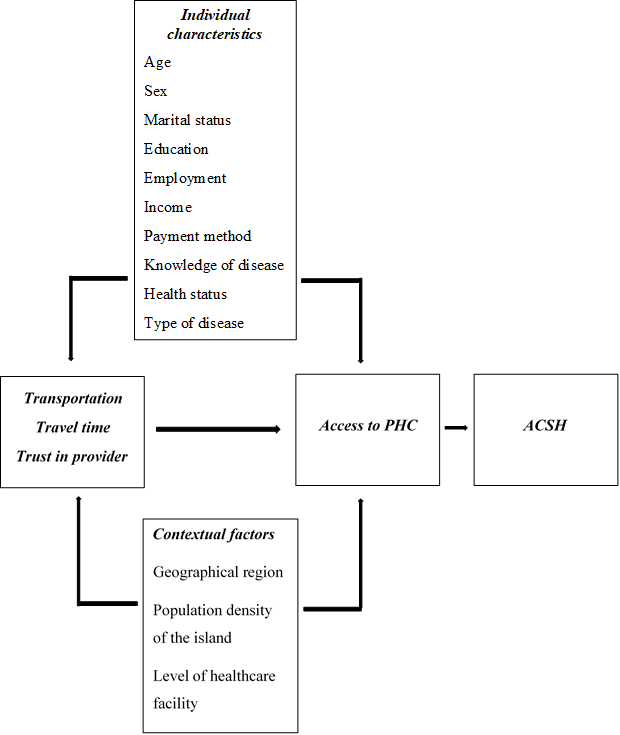
\includegraphics[width=0.90\textwidth]{3TModel.png}
\end{figure}

The conceptual model explains how individual's perceived levels of access to PHC services, in the Maldives influences ACSH. These levels of access to PHC may be determined by transportation, travel time, and trust in provider. The conceptual categories are grouped into main explanatory variables - transportation, travel time, and trust in provider. The covariates are individual characteristics - age, sex, marital status, employment, income, education, payment method, type of disease, health status, and knowledge of disease; and contextual factors - geographical region, population density of the island, and type of healthcare facility. 

The Andersen's behavioural model of families use of health services is used as a framework to guide the selection of variables for the conceptual model -Figure~\ref{f4}. Andersen's behavioural model reflects the systematic use of healthcare services by families through a measure of equitable access to medical care. The theory stresses on demographic characteristics and need factors to promote and develop policies that facilitate the utilisation of healthcare services \cite{andersen1968behavioral}. The predisposition of demographic factors, social structure and health beliefs with enabling resources either facilitate or hinder individual's use and need for care. Equitable access tends to occur when one's demographic characteristics and need factors account for use of healthcare services. Inequitable access tends to occur when one's social structure, health belief and enabling factors inhibit access to medical services \cite{andersen1995revisiting}. 

The three organising principles of Andersen's behavioural model predisposing, enabling, and need variables (refer to topic 1.9) that operate both under societal situations loosely termed as "contextual factors" which denote how they operate at system levels; and within individual agencies loosely named as "individual characteristics" which features individual level variables are used to categorise the variables -table~\ref{table 1}. The predisposing - contextual factors are geographical region and transportation. The predisposing - individual characteristics are age, sex, marital status, employment, education, knowledge of disease, and trust in provider. Enabling - individual characteristics are income, travel time, and type of disease. Need - individual characteristics are type of disease and health status. Population density of the islands and levels of healthcare facilities are specific to Maldivian context and do not fit precisely to the Andersen's behavioural model. 
% Done -make the table human readable
% align the ampersands

\begin{table}[]
\centering
\caption{Contextual factors and individual characteristics and Andersen's behavioural model }
\label{table 1}
\resizebox{0.70\linewidth}{!}{
\begin{tabular}{|l|l|l|}
\hline
                    \textbf{\begin{tabular}[c]{@{}l@{}}Andersen's \\ behavioural\\ model\end{tabular}}       
                                                                                           & \textbf{\begin{tabular}[c]{@{}l@{}}Contextual\\   factors\end{tabular}}                       & \textbf{\begin{tabular}[c]{@{}l@{}}Individual\\   characteristics\end{tabular}} \\ \hline
\multirow{7}{*}{\textbf{\begin{tabular}[c]{@{}l@{}}Predisposing\\   factors\end{tabular}}} & \multirow{7}{*}{}                                                                             & Age                                                                             \\ \cline{3-3} 
                                                                                           &                                                                                               & Sex                                                                             \\ \cline{3-3} 
                                                                                           &                                                                                               & Marital status                                                                  \\ \cline{3-3} 
                                                                                           &                                                                                               & Employment                                                                      \\ \cline{3-3} 
                                                                                           &                                                                                               & Education                                                                       \\ \cline{3-3} 
                                                                                           &                                                                                               & Knowledge of disease                                                            \\ \cline{3-3} 
                                                                                           &                                                                                               & Trust in provider                                                               \\ \hline
\multirow{3}{*}{\textbf{Enabling factors}}                                                 & \multirow{3}{*}{\begin{tabular}[c]{@{}l@{}}Geographical region\\ Transportation\end{tabular}} & Income                                                                          \\ \cline{3-3} 
                                                                                           &                                                                                               & Travel time                                                                     \\ \cline{3-3} 
                                                                                           &                                                                                               & Payment method                                                                  \\ \hline
\multirow{2}{*}{\textbf{Need factors}}                                                     & \multirow{2}{*}{}                                                                             & Type of disease                                                                 \\ \cline{3-3} 
                                                                                           &                                                                                               & Health status                                                                   \\ \hline
\end{tabular}
}
\end{table}

\chapter{Literature} 

\section{Concept of access}

Access can be defined as an individual's opportunity to reach and obtain needed health care services \cite{levesque2013patient}. In general, authors agree access to health care is the interface between service providers and actual health care users. 

More recently, access has been conceptualised as individual's opportunity to satisfy health care needs \cite{levesque2013patient}. It is related to how service providers manage approachability, acceptability, availability, affordability and appropriateness \cite{levesque2013patient}. These variables interact with the individual's ability to perceive, seek, reach, engage, and pay for healthcare services. It is assumed that these factors have an impact on each other. For example: though cost of services are affordable, one's ability to pay for those services can affect the health seeking behaviour.

Cost, access, and quality are three unique determinants of health system performance that are distinguished from each other \cite{donabedian2002introduction}. Cost refers to the monetary and time-wise expenses associated with providing or receiving care; access to care relates to how care reaches patients or how patients find out and reach care providers; and quality of care concerns the mechanics of care provided. In defining access, Donabedian emphasised on spatial characteristics - friction of space such as distance to healthcare provider, cost and availability of appropriate transportation; organisational characteristics such as opening times; economic factors - possession of insurance coverage and individual's income; social and cultural factors including one's religion and  ethnicity as determinants in access to health care services \cite{donabedian2002introduction, donabedian1973aspects}.

Mooney reserves the term access as an interface between demand and supply of health care services \cite{mooney1983equity}. Mooney found provider or supplier characteristics including availability of appropriate health care services, cost of services, and geographic location to be an influence for access to health care services. Association of provider characteristics and access to healthcare are supported by Bodenheimer and Freeborn \cite{bodenheimer1970patterns,freeborn1973evaluation}. Mooney further explains how access to healthcare is a product of demand factors including knowledge, attitude, skills, and care practices \cite{mooney1983equity}. It is argued that a fit between attributes of health services and ability to consume health care services enhance access to healthcare services for the population \cite{mooney1983equity}. 

Access can be studied through outcome indicators such as satisfaction scores, and utilisation rates \cite{rogers1973american}. The satisfaction scores are based on the health care services provided by the supplier and expectation of the clients or patients in reaching and utilising these health care services in proportion to their needs. It is argued that utilisation rates can profoundly depend on patient's satisfaction with operational characteristics of the health care provider such as emergency department waiting times \cite{morgan2015demographic}.

\section{Selection of ambulatory care sensitive conditions}

The concept of ACSH was first introduced in the late 1980's by John Billings of New York University to explain the variations in access and utilisation of health care services by vulnerable populations \cite{WHO:health:hospitalizations}. The initial catalogue of conditions suggested by Billings and colleagues were concentrated on those in the United States, and later streamlined by Germany, Portugal, Spain and United Kingdom for the European context \cite{WHO:health:hospitalizations}. 

The five ACSCs that will be used for this study (asthma, diabetes, COPD, CHF, and hypertension) have appeared in various lists including those published by Caminal and others, King Fund, Bardsley, and The Agency for Healthcare Research and Quality (AHRQ) \cite{caminal2004role,The:Kings:Fund,bardsley2013secondary}. Bardsley and colleagues classify ACSCs into three main categories: acute, chronic, and preventable conditions \cite{bardsley2013secondary}. Acute conditions are classified based on hospitalisations due to failure in early detection of symptoms leading to a more acute condition. Chronic conditions are those where hospitalisation is required due to failure or inappropriate management of long-term chronic conditions. Preventable conditions refer to hospitalisations as a result of inappropriate coverage of PHC leading to disease outbreaks. Caminal and others' list of ACSCs focuses on acute non-communicable conditions that do not usually require emergency hospital admissions and occurrence of acute complications \cite{caminal2004role}. Camnial and others have eliminated hospitalisation for communicable diseases in their list. The King Fund has published a list of 19 conditions with similar focus \cite{The:Kings:Fund}. AHRQ identifies 16 ACSCs as conditions for which proper outpatient care and early intervention prevents need for hospitalisation, complications, and more acute diseases \cite{guide:AHRQ:2001}. The Organisation for Economic Co-operation and Development (OECD) reports on common five ACSCs since 2007 \cite{WHO:health:hospitalizations,OECD:Data:countries}. Similar conditions have come up in WHO report to assess health services delivery performance with ACSH in Europe \cite{WHO:assess:acsh}. Additionally, these conditions have appeared in many other studies \cite{ansari2012patient,magan2011hospitalizations,ansari2006access,laditka2003hospital,foland2000avoidable,ricketts2001hospitalization}. 

\section{Ambulatory care sensitive hospitalisation as a proxy measure of access to primary health care}

ACSH is an accepted proxy measure of access to PHC \cite{10.1093/eurpub/cks053,ansari2012patient,magan2011hospitalizations,laditka2005more,WHO:assess:acsh,walker2013hospitalization,laberge2017hospitalizations,cecil2016primary}. This has been endorsed by United states Institute of Medicine\cite{millman1993access} and Agency for Healthcare Research and Quality (AHRQ) \cite{guide:AHRQ:2001}. AHRQ verified the reliability of it in terms of construct validity, precision and minimum bias. Ansari studied the validity of ACSH using the AHRQ framework as a measure of access to PHC \cite{ansari2007concept,guide:AHRQ:2001}. Critical interpretive synthesis was used to generate qualitative and quantitative evidence. The main finding of the study indicated the validity of ACSH as a proxy measure of access to PHC. Ansari found that ACSH can be used by policy makers and planners to monitor health services to pin point gaps in health systems. It can help to explore access barriers to PHC services. ACSH were also found to serve as a tool to evaluate effectiveness of interventions to improve access to PHC. It can contribute to analysing health care system to improve efficiency such as cost efficiency and improvement in population health. Finally, ACSH can be used to identify communities with greater access issues in comparison to areas with less access issues or in comparison to any other reference such as demographics. Muenchberger and Kendall described the usefulness of the measure \cite{muenchberger2010predictors}. They found that ACSH can be used to identify the focus areas to improve PHC access and quality of care. This is in terms of disease management, support services, service delivery, infrastructure and economic opportunities.  

ACSH, also known as a potentially preventable hospitalisation, is a hospital admission for ACSCs that under most circumstances should have been managed on an outpatient basis \cite{porter2007avoidable,weeks2016rates}.
The rationale for using ACSH as an indicator is that outpatient care of ACSCs can reduce the risk of hospitalisation through patient education, antibiotics, pharmaceuticals, and other treatments \cite{laditka2009health}.

It is argued that communities with higher rates of ACSH are considered to have impaired access to PHC services \cite{ansari2012patient,ansari2006access,laditka2003hospital,bindman1995preventable,billings1993impact,millman1993access}. This means that greater access to preventive care is associated with lower rates of ACSH. If patients with ACSCs were to visit their GPs regularly and on time, receive medicines and care and carried out lifestyle changes; then, even though these conditions might otherwise be associated with life threatening risks, hospital in-patient care and complications could be avoided when treated in the community. A system with high rates of ACSH, tells us that either people use less GP services, or that the system fails to provide adequate services. In both situations, patients have less access to PHC. This was supported by Ansari and colleagues \cite{ansari2006access}. Ansari and colleagues found that access is associated with ACSH $(R^2=0.29;p=0.001)$. The estimated co-efficient -20.64 of the study showed that every increment in level of access, reduced the ACSH by 20.64 per 1000 persons. A similar study by Bindman and colleagues found that communities in which people reported impaired access to PHC services for five chronic ambulatory sensitive conditions was negatively associated with higher rates of hospitalisations - $R^2=0.50;p<0.001$ \cite{bindman1995preventable}.

\section{Factors associated with access to primary health care and ACSH}

Ansari found that ACSH indicates the factors determining individuals' access to effective and timely PHC \cite{ansari2007concept}. Specifically, it was found that socio-economic factors explain variations in ACSH. Other factors that contribute to these variations include demographics, rurality of region, health system factors, prevalence of conditions, lifestyle factors, environment, adherence to medication, tendency to seek care, and severity of disease or condition \cite{ansari2007concept}. In addition to this, Mohseni argues that low trust in health care provider leads to poor self-rated health and hinders access to health care in terms of tendency to seek health care when needed \cite{mohseni2007social}. Further, findings by Shayo and others suggest that access and utilisation of public and private health care facilities are associated with level of trust in provider. This trust reflects perceived level of satisfaction with provider-client interaction \cite{shayo2016access}. 

Thomas and colleagues found that income, employment, and race are major contributors for lack of health insurance and failure to seek ambulatory care \cite{ricketts2001hospitalization}. The results did not show a high degree of correlation to health care resources such as physician supply. Therefore, Thomas and others argue that reduction in ACSH does not only require structural changes but changes in both structural and general economy for better access to PHC. In contradiction to findings of Thomas and colleagues, Ladhika and others later found that physician supply is related to PHC access in urban areas for ages between 18 to 64 years $(p<0.0001)$ \cite{laditka2005more}. 

It has also been reported that people with chronic conditions domiciled in rural areas are less likely to receive effective preventive services compared with those in urban areas \cite{casey2001rural}. Rural residents are more likely to have impaired health, disabled, uninsured, financially disadvantaged and incur travel burdens to obtain health care \cite{probst2004person,laditka2007health,laditka2009health,ziller2006out}. This report has been consistent over the years as rurality was also found to increase the ACSH in the US \cite{basu2014small}, Canada \cite{balogh2013factors} and Germany \cite{burgdorf2014potentially}. This is said to be related to the longer time of travel to hospitals. Report has shown that health care providers might admit patients and prevent them from travelling a great distance which could have an adverse effect on the conditions they came with \cite{laberge2017hospitalizations}. Some studies did not find any association between travel time and avoidable hospitalisation \cite{friedman2001health,magan2011hospitalizations}, while another study found a positive association \cite{bermudez2004organizational} . Magán and colleagues \citeyear{magan2011hospitalizations} reported that proximity to hospitals increased the frequency of ACSH leading to less use of PHC. While Balogh and colleagues \citeyear{balogh2013factors} reported that visits to a primary care physician was associated with an increased likelihood of being hospitalised for an ACSC. 

Wallace and colleagues found that 3.6 million Americans do not have access to health care as a result of lack of transportation services \cite{wallace2005access}. It was higher among females who come from underprivileged background with less education. It was also higher among older adults than younger ones. Findings by Arcury and colleagues reported that having transportation is an enabling factor to access health care services \cite{arcury2005access}. They found that those with personal transportation, transportation support by family and friends, and access to public transportation services were more likely to access health care services. Timyan and collegues later suggested that one's ability and willingness to seek health care are low when distance increases and transportation is limited; this is more specific to women \cite{timyan2018access}. 

Studies in Spain and the Netherlands reported that the rate of avoidable ACSH decreased with increasing available income \cite{magan2011hospitalizations,paul2018admissions}. They found out that socioeconomic factors were majorly responsible for patients’ access to PHC thereby influencing the rate of ACSH. In the US, lower supply of PHC physicians in some regions had a higher rate of ACSH \cite{laditka2005more}. In contrast, Balogh and colleagues \citeyear{balogh2013factors} did not find this association in their study. Magán and colleagues \citeyear{magan2011hospitalizations} posited that high physician workload could lead to poorer quality of health care due to the limited time available for consultation and resolution of health problems.

In addition to appropriate physician supply as a health care structural change suggested by Ladhika and others is different to Thomas and colleagues \cite{laditka2005more}, there are many other structural factors that determine the individuals access to effective and timely PHC. These variety of factors were recognised in a book published by Institute of Medicine. These include: patients waiting times for appointments and outside consultation rooms; patients perceived satisfaction level with medical staff communication to patients; patients interaction with administrative staff such as receptionist; accessibility to services including travel time, distance, and proximity of services; availability of PHC services including working hours, after hours, and weekends; linguistic and cultural compatibility of patient and doctor; and quality of services \cite{millman1993access}.

\chapter{Methods}

\section{Study design}

I have chosen to conduct:

\begin{itemize}
    \item A cross-sectional survey
    \item Case control study nested within a cross-sectional survey 
\end{itemize}

I will test the association between transportation, travel time, and trust in provider and self-reported access to PHC services in the Maldives by cross-sectional survey. Then I will construct a measurement as to how people were able to access PHC. I will use a median cut-off score to define low verses high self-reported access. Using this measurement low and high level of self-reported access, I will assess the association between self-reported access to PHC services in the Maldives and risk of ACSH. This will be done on the basis of the case control study where cases will be people who were hospitalised with consequences of ACSCs and controls will be who have not been hospitalised for ACSCs.

%Done: YOu cannot learn anything about an entire population 
% from a one-time cross-sectional survey, if anyone has written
% this (assuming you correctly interpreted levein2006study), that is wrong and you must 
% critique!! 
% Cross-section surveys provide a rapid and relatively inexpensive snapshot of the 
% prevalence of a problem. In your case, the issue is "access to primary health care in
% The Maldives. 
% So what? Cohort studies do that as well? Why did  you not choose a cohort study approach?
% A case control study will allow you to assess the likelihood of the risk of lower levels 
% of access to primary care on risk of ACSH relatively inexpensively and rapidly

\section{Study population and sample}

\subsection{Population - inclusion and exclusion criteria}

The study population is situated in the Maldives. Population aged 20 years and above with ACSCs from five regions have the probability of inclusion in the sample. Hospitals are selected based on population density of the islands and type of healthcare facility from five administrative divisions.

Individuals aged below 20 years will be excluded from the study. Since the data requires participants to recall past incidents, patients diagnosed with cognitive disorders and mental retardation will be excluded from the study. Patients admitted in rehabilitation centres and institutionalised populations such as military bases and prisons will be excluded from the study due to restrictions in paperwork that may apply. Populations living in foreign countries at the time of survey will be excluded from the study due to difficulties that might arise in reaching and communicating with them. These populations will be given a final weight of zero. They would not be counted for weighted estimates.

\subsection{Sample}

\subsubsection{Hospitals}

A total of 184 public hospitals were identified from twenty atolls of the Maldives, clustered into six administrative regions. These include Male', north, north central, central, south central, and south regions. Male' region is excluded from the study since major health care facilities (tertiary health care facilities) are located in capital city Male'. 

Nineteen hospitals of primary units are estimated in a convenience proportion of 1:10 - see table~\ref{f5}. This is above 10\% of total hospital units. It is to include maximum number of hospitals resources may allow, particularly funding. Also, this is to draw an operationally manageable sample; and for feasible, timely, and cost effective data collection. Hospitals were selected based on population density of the islands and hospital type. 

Population density of the islands are based on the proportion of low, average, and high populations in the region. Low populations are over sampled for the primary units due to great differences in number of people living in these islands, in comparison to islands with high populations. For example: In upper north, high category - Kulhudhufushi has a population of 9366, in comparison to low category - Hirimaradhoo 540. 

Hospitals in islands with populations above 5000 were considered for the high population category from each administrative division. These hospitals include: Kulhudhuffushi regional hospital, Naifaru atoll hospital, Gan regional hospital, and Hithadhoo regional hospital. Since islands of central region have populations below 5000, no hospital was selected for this category.

Hospitals in islands with populations between 1000 to 5000 were considered for average population category from each administrative division. These hospitals include: Dhidhdhoo atoll hospital, Un'goofaaru regional hospital, Rasdhoo atoll hospital, Veymandoo atoll hospital, and Viligili atoll hospital.

Hospitals in islands with populations below 1000 were considered for low population category from each administrative division. These hospitals include: Utheemu health centre, Hirimaradhoo health centre, Fainu health centre, Olhuvelifushi health centre, Mathiveri health centre, Felidhoo health centre, Kan'doodhoo health centre, Mundoo health centre, Kodey health centre, and  Kandhuhulhudhoo health centre. 

In selecting the population density proportions, the following were taken into consideration:

% Done: Use 'enumerated list', see my instructions above!

\begin{itemize}
  \item Populations relocated to other islands under population consolidation program, 
  \item Populations displaced to other islands due to tsunami,
  \item Newly inhabited islands under population consolidation program, and
  \item Populations inhibited in islands given for agricultural, industrial and tourism purposes. 
\end{itemize}

Hospital types were categorised into regional, atoll and island health centres. Regional and atoll hospitals belong to secondary care. Four regional hospitals were selected from north, north central, south central, and south region. These include Kulhudhuffushi regional hospital, Un'goofaaru regional hospital, Gan regional hospital, and Hithadhoo regional hospital. Five atoll hospitals were picked from all administrative divisions excluding Male'. They were Dhidhdhoo atoll hospital, Naifaru atoll hospital, Rasdhoo atoll hospital, Veymandoo atoll hospital, and Viligili atoll hospital. 10 health centres from all regions were added to the sample. These include Utheemu health centre, Hirimaradhoo health centre, Fainu health centre, Olhuvelifushi health centre, Mathiveri health centre, Felidhoo health centre, Kan'doodhoo health centre, Mundoo health centre, Kodey health centre, and  Kandhuhulhudhoo health centre.    

\begin{table}[H]
\centering
\caption{Selected hospital units}
\label{f5}
\resizebox{0.80\linewidth}{!}{
\begin{tabular}{|c|c|c|c|c|c|}
\hline
\textbf{Region} & \textbf{\begin{tabular}[c]{@{}c@{}}Atolls\\ in the \\ region\end{tabular}}                & \textbf{\begin{tabular}[c]{@{}c@{}}Atolls \\ hospitals\\ belong to\end{tabular}} & \textbf{\begin{tabular}[c]{@{}c@{}}High\\ population\end{tabular}}                                                                               & \textbf{\begin{tabular}[c]{@{}c@{}}Average\\ population\end{tabular}}      & \textbf{\begin{tabular}[c]{@{}c@{}}Low\\ population\end{tabular}}                                       \\ \hline
North           & \begin{tabular}[c]{@{}c@{}}Haa Alif, \\ Haa Dhaalu, \\ Shaviyani\end{tabular}             & \begin{tabular}[c]{@{}c@{}}Haa\\ Alif, \\ Haa \\ Dhaalu\end{tabular}             & \begin{tabular}[c]{@{}c@{}}Kulhudhuffushi\\ regional \\ hospital\end{tabular}                                                                    & \begin{tabular}[c]{@{}c@{}}Dhidhdhoo\\ atoll hospital\end{tabular}         & \begin{tabular}[c]{@{}c@{}}Utheemu\\ health centre \\ \& \\ Hirimaradhoo \\ health centre\end{tabular}  \\ \hline
North central   & \begin{tabular}[c]{@{}c@{}}Baa,\\ Lahviyani, \\ Noonu, \\ Raa\end{tabular}                & \begin{tabular}[c]{@{}c@{}}Lahviyani,\\   Raa\end{tabular}                       & \begin{tabular}[c]{@{}c@{}}Naifaru\\ atoll \\ hospital\end{tabular}                                                                              & \begin{tabular}[c]{@{}c@{}}Un'goofaaru\\ regional \\ hospital\end{tabular} & \begin{tabular}[c]{@{}c@{}}Fainu\\ health centre \\ \& \\ Olhuvelifushi \\ health centre\end{tabular}   \\ \hline
Central         & \begin{tabular}[c]{@{}c@{}}Alif Alif,  \\ Alif Dhaalu, \\ Kaafu, \\ Vaavu\end{tabular}    & \begin{tabular}[c]{@{}c@{}}Alif\\ Alif,  \\ Vaavu\end{tabular}                   & None                                                                                                                                             & \begin{tabular}[c]{@{}c@{}}Rasdhoo\\ atoll hospital\end{tabular}           & \begin{tabular}[c]{@{}c@{}}Mathiveri\\ health centre\\ \& \\ Felidhoo \\ health centre\end{tabular}     \\ \hline
South central   & \begin{tabular}[c]{@{}c@{}}Dhaalu,\\ Faafu, \\ Meemu, \\ Thaa, \\ Laamu\end{tabular}      & \begin{tabular}[c]{@{}c@{}}Thaa,\\ Laamu\end{tabular}                            & \begin{tabular}[c]{@{}c@{}}Gan\\ regional \\ hospital\end{tabular}                                                                               & \begin{tabular}[c]{@{}c@{}}Veymandoo\\ atoll hospital\end{tabular}         & \begin{tabular}[c]{@{}c@{}}Kan'doodhoo\\ health centre \\ \& \\ Mundoo \\ health centre\end{tabular}    \\ \hline
South           & \begin{tabular}[c]{@{}c@{}}Gaaf Alif, \\ Gaafu dhaalu, \\ Gnaviyani, \\ Addu\end{tabular} & \begin{tabular}[c]{@{}c@{}}Gaaf\\ Alif, \\ Addu\end{tabular}                     & \begin{tabular}[c]{@{}c@{}}Hithadhoo\\ regional \\ hospital\end{tabular}                                                                         & \begin{tabular}[c]{@{}c@{}}Viligili\\ atoll hospital\end{tabular}          & \begin{tabular}[c]{@{}c@{}}Kodey\\ health centre \\ \& \\ Kandhuhulhudhoo \\ health centre\end{tabular} \\ \hline
Male'           & Male'                                                                                     & Male'                                                                            & \begin{tabular}[c]{@{}c@{}}None\end{tabular} & None                                                                       & None                                                                                                    \\ \hline
\end{tabular}
}
\end{table}


\subsubsection{Respondents}

\textbf{Respondents for cross-sectional study:} A population of 71940 was estimated to have diabetes, COPD, asthma, and cardiovascular diseases in the Maldives \cite{IHME:Data:Maldives}. The estimated sample size was derived by computing a minimal sample size required for accuracy on OpenEpi website \cite{open:epi:2013}. A sample of 450 was estimated with a confidence level of 95\% and power 80\% with prevalence odds ratio of 2 assuming that those with low levels of transportation, long travel time, and less trust in the provider are two times more likely to have low level of access to PHC. An additional 20\% samples were added assuming that not every potential respondent will participate in the study. This rounds to a figure of 540 samples. 
  
The sample units for the regions will be proportionately allocated based on the number of patients with ACSCs identified from the hospitals from that particular region. A simple random sampling technique will be used to assign the sample units. This will be achieved through a lottery system using a sampling frame. The potential respondents chosen through the lottery, will be included in the sample. This will allow every potential subject to have equal probability of inclusion. 

\textbf{Respondents for case control study:} The cases for case-control study are patients with ACSCs hospitalised for consequences of the conditions (cerebrovascular accident - intracerebral haemorrhage and ischemic stroke, respiratory failure, chronic heart failure, retinopathy, renal failure, and gangrene). The controls for case-control study are patients with ACSCs not hospitalised for consequences of the conditions. The maximum number of cases identified by cross-sectional survey will be studied in a ratio of 1:1 with controls that will be identified from the cross-sectional study. Simple random sampling will be used to assign the controls for the case control study.

%Done 
% No case two now - I did not understand case 2, what is that supposed to mean????
% Indicate the plans for the cross-section survey first. On what basis will you select the
% sample size of cross-section survey? Use OpenEpi website to estimate that figure
% OpenEpi is not an Open Source software, it is a free website, cite the website
% State the estimated Odds ratio (this is referred to as Prevalence Odds Ratio
% What you are attempting to do in the case control study is you are trying to assess the
% likelihood of high/low access among the hospitalised versus the community controls AND
% you are trying to find the relationship between travel, transport, and trust levels 
% and high/low access. 
% Then state an arbitrary value of the Odds Ratio and calculate the sample size
% Done 15% - To calculate the sample size, you will need to state what percent of people / who HAVE any or more of a combination of the five diseases and are NOT hospitalised / but access primary care. This population is the assumed percentage of people who / have hypertension, diabetes, chf, copd, asthma and access health services? / If you are not sure what that number is, think of several percentages, say, 5, 10, 15 ... / and on that basis, run the calculations and settle on a feasible value
% Your real estimates can differ and that is alright. But you will need to 
% justify your calculations
%Define the cases and controls
%So, define what you mean by high or low levels of access. You can state for example,
% you will construct a composite score from say 3 or 4 items from the survey you will
% administer to quantify a self-reported level of access; then state that
% you will use a median cut-off score to decide high versus low level access
% Also state that you will use this score as a continuous variable

\section{Instrument of observation}

A standardised questionnaire will be used to elicit the information required - refer to appendix 1. The questionnaire will be interviewer-administered (face-to-face). It will be delivered in English and Dhivehi languages. The questionnaire translation will be carried out by 2 lecturers of Faculty of Arts of the Maldives National University (MNU) refer to appendix 3. The researcher will compare the original English version and the translated version and the process will be repeated till maximum match is achieved. 

%Done
% Please use simple English sentences. 
% If you meant that you will draft  your study instrument in two languages, English and 
% Dhivehi, write that as a simple sentence (Noun-verb-object: e.g., "The student will develop 
% a questionnaire in English and Dhivehi language". 
% "To ensure maxium questions are answered" suggests coercion, you will find it difficult to
% pass Ethics if you write these things. Write what you will do. Write, "The questions will be interviewer-administered". Then write, "Members from the Faculty of Arts (how many members will be involved?) who have no knowledge of the English version will back translate the Dhivehi version to English language. The researcher will compare the original English version and the translated version and the process will be repeated till maximum match is achieved. "To ensure resembles original document" suggests cheating.
% Canterbury Human Ethics Committee cannot comment on the translation! They can comment on the
% Ethics of your research. You will need to test the quality of the translation! It is an 
% iterative process.

The core of the questionnaire consists of four main components: sample adult verification (SAV 100 to 111); socio-demographics (SOC 112 to 117); health information (HEI 118 to 125); and health service utilisation and patient experience (HSU 126 to 157). The questionnaire core sections address the variables in the conceptual model - Figure~\ref{f4}. The designated core sections are titled with three digit letter codes. The number identifies the question order in each core section. The questions SOD 112 to HEI 124, HSU 126 to HSU 140, HSU 144 to 148, and 153 to 157 are adapted from already validated questionnaires. Questions HSU 125, HSU 141-143, and HSU 147-152 are constructed to capture transport, travel time, hospitalisation, trust in provider, and access within and between islands. 

To validate the questionnaire, a face and content validity and pilot study will be conducted. For face validity, the questionnaire will be read by two study subjects to check the syntax and how easy it is to understand the questionnaire. For content validity, questionnaire will be read by two experts to ensure that the contents capture the topic under investigation. A pilot study will be conducted for 5\% of the total population - 27 potential respondents. This is to establish appropriate delivery of questions. Content validity, face validity and pilot study will check for errors, misleading and confusing questions. 

%Done
% Face validity is the syntax and how easy to fill in and understand the questionnaire
% Content validity refers to whether the questionnaire can 'capture' the contents of the
% research. These are two different things
% What do you mean by this??

To test reliability of the questionnaire, Chronbach's alpha and omega will be calculated for each of the construct in the questionnaire - travel time, transportation, trust in provider, and self-reported access. A value greater than 0.80 will indicate good internal consistency. 
%Done
% Cronbach's alpha is not a single measure. Cronbach's alpha is either calculated for an 
% entire questionnaire when the aim is to capture only ONE construct. In your case, you 
% are studying AT LEAST four constructs: construct one - travel, construct two - %transportation, 
% construct three - trust, construct four - self-reported access.
% You must write that you will measure Cronbach's alpha and omega for EACH of these
% four constructs 

\subsection{Core sections}

The four core sections collect information about main topic areas in Table~\ref{f8}. These include sample adult verification, socio-demographics, health information, and health service utilisation and patient experience.

\begin{table}[!ht]
    \centering
    \begin{tabular}{@{}lllrl@{}}\toprule
     Topic area                     & Topics    \\ \midrule
     Core 1 - Sample adult verification  & Geographical region, and population density of the island, \\    
     Core 2 - Socio-demographic factors  & Sex, age, marital status, education, employment,  \\  
                                         & and income \\
     Core 3 - Health information         & Health status, type of disease, and knowledge of disease\\ 
     Core 4 - Health service utilisation & Level of healthcare facility, travel time, public transport, \\
                                         & payment method, and trust in provider \\\bottomrule
    \end{tabular}
    \caption{Core sections of the questionnaire}
    \resizebox{0.50\linewidth}{!}{
    \label{f8}
}
\end{table}

To capture the topics in table~\ref{f8} questions from several questionnaires are adapted. They are as follows:

The New Zealand Health Survey 2016-2017 (NZHS) is adapted to capture information relevant to employment, income, knowledge of disease-diabetes/CHF, type of health facility, trust in provider, transport, and payment method \cite{NZHS:Newzealand:2017}. These questions include 116-117, 120-121, 124, 126-131, 133-138, 140, 144-145, 154, and 156. NZHS provides information about health and well-being of people of New Zealand. The survey consists of two core parts: child questionnaire and adult questionnaire. For this particular study, only questions from adult questionnaire are being adapted. NZHS was conducted in 1992-1993, 1996-1997, 2002-2003, 2006-2007, and 2016-2017. 

National Health Interview Survey (NHIS), by Centres for Disease Control and Prevention (CDC), United States is adapted to capture information relevant to sex, education, health status, and knowledge of disease-hypertension/COPD/asthma \cite{Centre:disease:control}. These questions include 112, 115, 118, 119, 122, and 123. The NHIS collects data on a broad range of health topics for non-institutionalised population of United States since 1957. The questionnaire tool is updated and field tested periodically. 

The survey instruments utilised in national survey on access to medical care by Ronald M. Andersen and Lu Ann Aday is extracted from inter-university consortium for political and social research (ICPSR) by University of Michigan - ICPSR 8244 study tool \cite{Andersen:questionnaire:1982}. This is adapted to capture travel time, and transport. These questions include 132, 147, 148, 153, and 155. The purpose of the national survey on access to medical care was to update 1976 data on access to medical care in the United States associated with individual and healthcare system level variables. The questionnaire tool for national survey on access to medical care - ICPSR 8244 is used in 1953, 1958, 1964, 1971, 1976 and 1982 in the United States to measure access to medical care. 

Maldives Demographic and Health Survey 2016-2017 (MDHS) is adapted to capture information relevant to age and sex \cite{Maldives:demographichealthsurvey:2017}. These questions include 113-114. MDHS is designed to provide information about reproduction, contraception, pregnancy, postnatal care, immunisation, child health, nutrition, marriage, sexual activity, socio-demographics, health issues, and domestic violence that are crucial for policy making, program planning, and attainment of sustainable development goals in the Maldives. The 2016-2017 MDHS is the second demographic and health survey conducted in the Maldives in collaboration with demographic and health survey program. 

Victorian population health survey is adapted to capture access - question 157 \cite{Victorian:healthsurvey:2017}. Victorian population health survey collects valid health information that is applied for policy development and strategic planning over 18 years. Similar question is used by Ansari and colleagues \cite{ansari2006access} to capture in overall, how difficult it is for the respondent to get medical care when he/she need it. The participants rated this on a 5 point scale listed numerically from highest to lowest.  

\section{Data sources}

\subsection{Hospital records}

Hospital patient data from selected hospitals of north, north central, central, south central, and south regions of the Maldives will be collected to identify the potential respondents diagnosed with ACSCs. Following the cross-sectional survey, hospital records will be collected to verify whether individuals who report they have been hospitalised for cerebrovascular accident (intracerebral haemorrhage and ischaemic stroke), respiratory failure, chronic heart failure, retinopathy, renal failure, and gangrene in the survey are hospitalised for these conditions. This is to identify the cases for case control study who have been hospitalised for consequences of ACSCs.

The information can be accessed when appropriate permission from Ministry of Health (MoH) is obtained. A formal online request will be mailed to policy planning and international health division (PIH) of the MoH, after ethics approval. MoH will request public health sections of the hospitals to release requested data, once approved. 

\subsection{Survey data}

Potential respondents from five regions of the Maldives will be invited to participate voluntarily in a survey. Survey deployment method will be face-to-face or telephone. This will depend on the preference of the potential respondents. 

Survey will be carried out by three field workers who will be directed by the researcher. They will work under a contractual agreement with the support of MoH and public health divisions of the hospitals. However, field workers will be independent to these departments and would not have any direct connection with MoH. Field workers will be selected through an interview process. Priority will be given to applicants who collected national demographic and health survey data 2017. 

Field workers will receive training on how to conduct the survey. This includes questionnaire administration, communication, entry of responses to laptop computer or tablet, cultural competency, and field procedures. Training will be targeted to familiarise field workers with the questionnaire. Demo presentations and field practice by each field worker will be carried out to ensure that they are prepared for field work. This will also minimise the differences in responses by applying same standardised technique in asking the questions. The field workers will be guided on how to keep appropriate pace, and the respondent focused. Additionally, field workers will be strictly instructed to treat the participants ethically and equally. 

Field workers will provide an information card to the potential respondents and check whether the respondents understand the information provided - refer to appendix 2. Field workers will make respondents aware that they can withdraw from the survey at any stage; do not have to answer every question; can ask questions about the study at any time; and contact the researcher for further information. Once field workers clarify any doubts or questions about the survey, they will obtain consent from the participants.  Participants will sign the consent paper prior to answering the questions. Field workers will instruct the participants to take time before answering questions and to provide accurate response to the best of his/her of knowledge. 

Confidentiality of participants will be assured by using participants study codes on data documents. Respondents will be assured that the usage of information is for research purposes.

Field workers can make up to four visits or calls on different hours of the day and on different days of the week to decide a potential participant is a 'non-contact'. Field workers will first make two visits or calls in the first month from the start date of the survey. If a potential respondent is not able to be contacted, they will make another visit or call after two weeks gap. This will be followed until fourth visit or call is over. The initial two visits or calls would be recorded between at least four hours of gap, to be considered as a new event. This will help to contact the potential participants who might not be in the island or in contact at the initial visit or call for data collection.

\section{Analysis of data}

Data analysis consists of the following steps:

\subsection{Pre-processing data}

I will use R statistical program to analyse the data. I will check computer grid to determine accurate entry of all responses. The data cleaning will include identifying inaccurate records, duplicate entries, missing values, and outliers to remove major errors and inconsistencies in data. I will conduct an inspection for scores outside the accepted range. This is to identify the outliers. An outlier is a data point that significantly differs greatly from the trends expressed by the other values for continuous variables in the data set. An outlier will be considered as any value that lies 1.5 times outside the inter-quartile range on either side. The inter-quartile range is a measure of statistical dispersion. To detect outliers for categorical data, I will produce single variable frequency distribution tables with counts. This will identify values that are beyond the reasonable ranges. I will check for missing values for all variables under study. I will consider removal or imputation if missing values exceeds more than 10\% for any data point. I will use explicit modelling approach for imputation \cite{kwak2017statistical}. According to Kwark and Kim \citeyear{kwak2017statistical} explicit modelling approach assumes that "variables have a certain predictive distribution and estimates the parameters of each distribution, which is used for imputation" (p.407). There are various imputation methods that can be followed by explicit modelling approach. They are regression, predictive-regression, assumption of distribution, mean, median, probability, and ratio. I will consider mean imputation or regression imputation for continuous variables; and mode imputation or regression imputation for categorical variables. 
  
\subsection{Univariate analysis}
 
I will present separate tables for continuous and categorical data. To describe the trends in continuous data of a single variable, I will compute mean value and inter-quartile range. The mean value will provide average number. Inter-quartile range will provide the difference between the third and first quartile. I will present the 25th percentile, the median, the 75th percentile, and the maximum value. I will present categorical data in total counts and percentages. 

\subsection{Bivariate  analyses}

One outcome variable of this study is 'self-reported access'. Self-reported access is a binary variable - low and high. I will use a median cut-off score to define high verses low self-reported access. The other outcome variable of this study is hospitalisation. This is also a binary variable - hospitalised and not hospitalised. The main explanatory variables are transportation, travel time, and trust in provider. The covariates are contextual factors and individual characteristics. Contextual factors are geographical location, population density of the island, and type of health care facility. Individual characteristics are age, sex, marital status, employment, income, education, payment method, type of disease, health status, and knowledge of disease. I will use binary logistic regression to conduct bivariate analyses. Bivariate analyses will identify: 1) the association between explanatory variables and covariates and self-reported access and 2) the association between self-reported access and risk of hospitalisation. Estimates of p-values will determine the variables to be tested in multiple regression models. I will use p-value cut-off point 0.05 to indicate statistical significance between the variables. 


\subsection{Multiple regression analyses}

Multiple logistic regression will quantify the best fit of variables. Multiple regression analyses will identify the association between transportation, travel time, and trust in provider and self-reported access to PHC in the Maldives after adjusting for other variables including age, sex, marital status, employment, income, education, payment method, type of disease, health status, knowledge of disease, geographical region, population density of the island, and type of healthcare facility. 

Multiple regression analyses will also identify the association between self-reported access to PHC in the Maldives and ACSH after adjusting for other variables such as transportation, travel time, and trust in provider, age, sex, marital status, employment, income, education, payment method, type of disease, health status, knowledge of disease, geographical region, population density of the island, and type of healthcare facility. 

I will examine the explanatory variables and covariates for multicollinearity. This is to identify the correlation between predictor variables under investigation. It will examine how collinear predictors under multiple regression models predict access to PHC and ACSH. Collinearity diagnostics may suggest changes to the model; if there is notable challenge to the model. The variance inflation factor (VIF) will quantify the severity of multicollinearity. I will remove the variables that cause multicollinearity issues from the regression if it exceeds VIF cut off point 10 \cite{neter1996applied}. If multicollinearity is relatively high the estimates for regression coefficient values and test of significance can be problematic; this can lead to type II error. 

 \section{Ethics approval}
 
 I will ensure the study meets all ethics requirements for the protection of human research participants in the Maldives. I will submit the ethics approval for the use of hospital in-patient data and survey data for research purpose to the University of Canterbury's Ethics Committee for research involving human participants. This is to justify the scientific soundness of the research without exposure to risk and misuse of data. All participants will consent to use their information for research with the assurance of name being removed that will be received from hospital records. They will be informed of their rights regarding participation in research. Research findings from the study will be sensitively reported using language that does not further disadvantage the participants. This approval will ensure independent ethical review of the research to safeguard the rights, health and well-being of the research participants.
 
 \section{Proposed structure of thesis}
 
Chapter 1 - Introduction and background

Chapter 2 - Ambulatory care sensitive conditions

Chapter 3 - Access to primary healthcare

Chapter 4 - Theoretical Background 

Chapter 5 - Methodology and methods 

Chapter 6 - Substantive analytical chapters 

Chapter 9 - Discussions 

Chapter 10 - Conclusions

\section{Work plan and time table}

The timeline presented is tentative and may change as the study progresses table~\ref{f10}. I expect to complete the study within the 3 years allowed. I will also develop and submit one paper for publication in each of the second and third years of the study. The journals in focus are Australian and New Zealand Journal of Public Health. A time line plan is presented below.

\begin{table}[H]
\centering
\caption{Proposed timeline for PhD study}
\label{f10}
\resizebox{0.60\linewidth}{!}{
\begin{tabular}{lll}
\hline
\multicolumn{3}{c}{\textbf{Propose timeline for the PhD study}}                                                                                                                                                                                                                                                                                          \\
\textbf{\begin{tabular}[c]{@{}l@{}}Time \\ period \\ (3 months)\end{tabular}}                                    & \textbf{Tasks}                                                                                                         & \textbf{Milestones to complete}                                                                              \\
\multirow{2}{*}{\textbf{\begin{tabular}[c]{@{}l@{}}1 \\ (Feb 18 \\ to \\ April 18)\end{tabular}}}                & \begin{tabular}[c]{@{}l@{}}Develop research \\ ideas.\end{tabular}                                                     & Research idea accepted.                                                                                      \\
                                                                                                                 & \begin{tabular}[c]{@{}l@{}}Undertake consultations \\ and form supervisory team.\end{tabular}                          & Supervision team formed                                                                                      \\
\multirow{4}{*}{\textbf{\begin{tabular}[c]{@{}l@{}}2 and 3\\ (May 18, \\ July 18 \\ to \\ Nov 18)\end{tabular}}} & \begin{tabular}[c]{@{}l@{}}Write initial research \\ proposal.\end{tabular}                                            & \begin{tabular}[c]{@{}l@{}}Relevant research materials \\ located\end{tabular}                               \\
                                                                                                                 & Begin writing background                                                                                               & \begin{tabular}[c]{@{}l@{}}Initial introduction and \\ background of the proposal \\ completed.\end{tabular} \\
                                                                                                                 & \begin{tabular}[c]{@{}l@{}}Submit progress note to \\ PG school\end{tabular}                                           & \begin{tabular}[c]{@{}l@{}}6 month progress note \\ achieved\end{tabular}                                    \\
                                                                                                                 & \begin{tabular}[c]{@{}l@{}}Literature searching and \\ reviewing\end{tabular}                                          & Relevant literature located                                                                                  \\
\textbf{\begin{tabular}[c]{@{}l@{}}4 \\ (Feb 19 \\ to \\ April 19)\end{tabular}}                                 & \begin{tabular}[c]{@{}l@{}}Further reading and writing of \\ research proposal\end{tabular}                            & \begin{tabular}[c]{@{}l@{}}Initial literature review and \\ methods section completed\end{tabular}           \\
\multirow{3}{*}{\textbf{\begin{tabular}[c]{@{}l@{}}5 \\ (May 19 \\ to \\ July 19)\end{tabular}}}                 & Finalising research proposal.                                                                                          & \begin{tabular}[c]{@{}l@{}}Submission of research \\ proposal\end{tabular}                                   \\
                                                                                                                 & Proposal Presentation                                                                                                  & Advance to Candidacy                                                                                         \\
                                                                                                                 & Application for ethics approval                                                                                    \\
\textbf{\begin{tabular}[c]{@{}l@{}}6 \\ (Aug 19 \\ to \\ Oct 19)\end{tabular}}                                   & \begin{tabular}[c]{@{}l@{}}Collection of hospital in-patient \\ data and survey data from\\  the Maldives\end{tabular} & \begin{tabular}[c]{@{}l@{}}Receive ethics approval & Data collection \\   completed\end{tabular}                                       \\
\multirow{2}{*}{\textbf{\begin{tabular}[c]{@{}l@{}}7 \\ (Nov 19 \\ to \\ Jan 20)\end{tabular}}}                  & Data analysis                                                                                                          & \begin{tabular}[c]{@{}l@{}}Data analysis ready for \\ possible journal \\ publication\end{tabular}           \\
                                                                                                                 & Writing of chapter 5 and 6                                                                                             & Chapter 5 and 6 draft                                                                                        \\
\multirow{3}{*}{\textbf{\begin{tabular}[c]{@{}l@{}}8 \\ (Feb 20 \\ to \\ April 20)\end{tabular}}}                & Thematic review of literature                                                                                          & Concepts definitions formed                                                                                  \\
                                                                                                                 & \begin{tabular}[c]{@{}l@{}}Revisit new themes and theories in \\ literature\end{tabular}                               & \begin{tabular}[c]{@{}l@{}}New literature incorporated \\ as needed\end{tabular}                             \\
                                                                                                                 & Begin writing final chapters                                                                                           & \begin{tabular}[c]{@{}l@{}}Writing chapter 2, 3, and 4 \\ continues\end{tabular}                             \\
\textbf{\begin{tabular}[c]{@{}l@{}}9 \\ (May 20 \\ to \\ July 20)\end{tabular}}                                  & Writing continiues                                                                                                     & \begin{tabular}[c]{@{}l@{}}Final drafts for chapter 2, 3, 4, \\ 5, and 6 completed\end{tabular}              \\
\multirow{2}{*}{\textbf{\begin{tabular}[c]{@{}l@{}}10 and 11 \\ (Aug 20 \\ to \\ Jan 21)\end{tabular}}}          & Findings examined                                                                                                      & \begin{tabular}[c]{@{}l@{}}Thesis argument from the \\ analysed data completed\end{tabular}                  \\
                                                                                                                 &                                                                                                                        & Final draft for chapter 9                                                                                    \\
\multirow{4}{*}{\textbf{\begin{tabular}[c]{@{}l@{}}12 \\ (Feb 21 \\ to \\ April 21\end{tabular}}}                & Continue write up                                                                                                      & \begin{tabular}[c]{@{}l@{}}Final drafts for chapter 1 \\ and 10 completed\end{tabular}                       \\
                                                                                                                 & Checking citations                                                                                                     & All chapters refined                                                                                         \\
                                                                                                                 & Organise proof reading                                                                                                 & Final draft ready                                                                                            \\
                                                                                                                 & Editing and finalising draft                                                                                           & Thesis submitted                                                                                             \\
\textbf{\begin{tabular}[c]{@{}l@{}}13 \\ (May 21 \\ to \\ July 21)\end{tabular}}                                 & Thesis examined                                                                                                        & Graduation (Dec 21)                                                                                         
\end{tabular}
}
\end{table}

\section{Budget}

Table~\ref{f11} indicates estimated cost for data collection. A total of 2,290 dollars will be personally funded. An additional 1500 dollars will be funded by the available student grants for PhD research purpose. 
\begin{table}[H]
\centering
\caption{Proposed budget for data collection}
\label{f11}
\resizebox{0.65\linewidth}{!}{
\begin{tabular}{lllll}
\textbf{\begin{tabular}[c]{@{}l@{}}Budget\\  item\end{tabular}}   & \textbf{}                                                        & \textbf{Quantity} & \textbf{Amount} & \textbf{Total (NZD)} \\
Travel by air                                                     & Kulhudhuffushi                                                   & 1                 & 150             & 150                  \\
                                                                  & Naifaru                                                          & 2                 & 150             & 300                  \\
                                                                  & Gan                                                              & 1                 & 150             & 150                  \\
                                                                  & Hithadhoo                                                        & 1                 & 150             & 150                  \\
                                                                  & Viligili                                                         & 2                 & 150             & 300                  \\
Travel by boat                                                    & Kulhudhuffushi                                                   & 1                 & 100             & 100                  \\
                                                                  & Dhidhdhoo                                                        & 1                 & 100             & 100                  \\
                                                                  & Utheemu                                                          & 1                 & 20              & 20                   \\
                                                                  & Hirimaradhoo                                                     & 1                 & 20              & 20                   \\
                                                                  & Naifaru                                                          & 2                 & 50              & 100                  \\
                                                                  & Un'goofaaru                                                      & 2                 & 20              & 40                   \\
                                                                  & Olhuvelifushi                                                    & 2                 & 20              & 40                   \\
                                                                  & Fainu                                                            & 2                 & 20              & 40                   \\
                                                                  & Rasdhoo                                                          & 2                 & 20              & 40                   \\
                                                                  & Mathiveri                                                        & 2                 & 20              & 40                   \\
                                                                  & Felidhoo                                                         & 2                 & 20              & 40                   \\
                                                                  & Veymandoo                                                        & 1                 & 100             & 100                  \\
                                                                  & Mundoo                                                           & 1                 & 10              & 10                   \\
                                                                  & Kan'doodhoo                                                      & 1                 & 20              & 20                   \\
                                                                  & Viligili                                                         & 2                 & 100             & 200                  \\
                                                                  & Kandhuhulhudhoo                                                  & 2                 & 20              & 40                   \\
                                                                  & Kodey                                                            & 2                 & 20              & 40                   \\
                                                                  & Male'                                                            & 0                & 0              & 0                  \\
\begin{tabular}[c]{@{}l@{}}Travel by\\   land\end{tabular}        & Gan                                                              & 1                 & 20              & 20                   \\
                                                                  & Hithadhoo                                                        & 1                 & 20              & 20                   \\
                                                                  & Male'                                                            & 0                & 0               & 0                   \\
\begin{tabular}[c]{@{}l@{}}Food and \\ accommodation\end{tabular} & \begin{tabular}[c]{@{}l@{}}Haa\\   Alif, Haa Dhaalu\end{tabular} & 4                 & 20              & 80                   \\
                                                                  & \begin{tabular}[c]{@{}l@{}}Lahviyani,\\   Raa\end{tabular}       & 4                 & 20              & 80                   \\
                                                                  & \begin{tabular}[c]{@{}l@{}}Alif\\   Alif,  Vaavu\end{tabular}    & 4                 & 20              & 80                   \\
                                                                  & \begin{tabular}[c]{@{}l@{}}Thaa,\\   Laamu\end{tabular}          & 4                 & 20              & 80                   \\
                                                                  & \begin{tabular}[c]{@{}l@{}}Gaaf\\   Alif, Addu\end{tabular}      & 4                 & 20              & 80                   \\
Tablet                                                            & 3 field workers                                                  & 2                 & 250             & 500                  \\
Field workers salary                                              & 28 days                                                          & 28                & 20              & 560                  \\
Total                                                             &                                                                  &                   &                 & 3540                
\end{tabular}
}
\end{table}

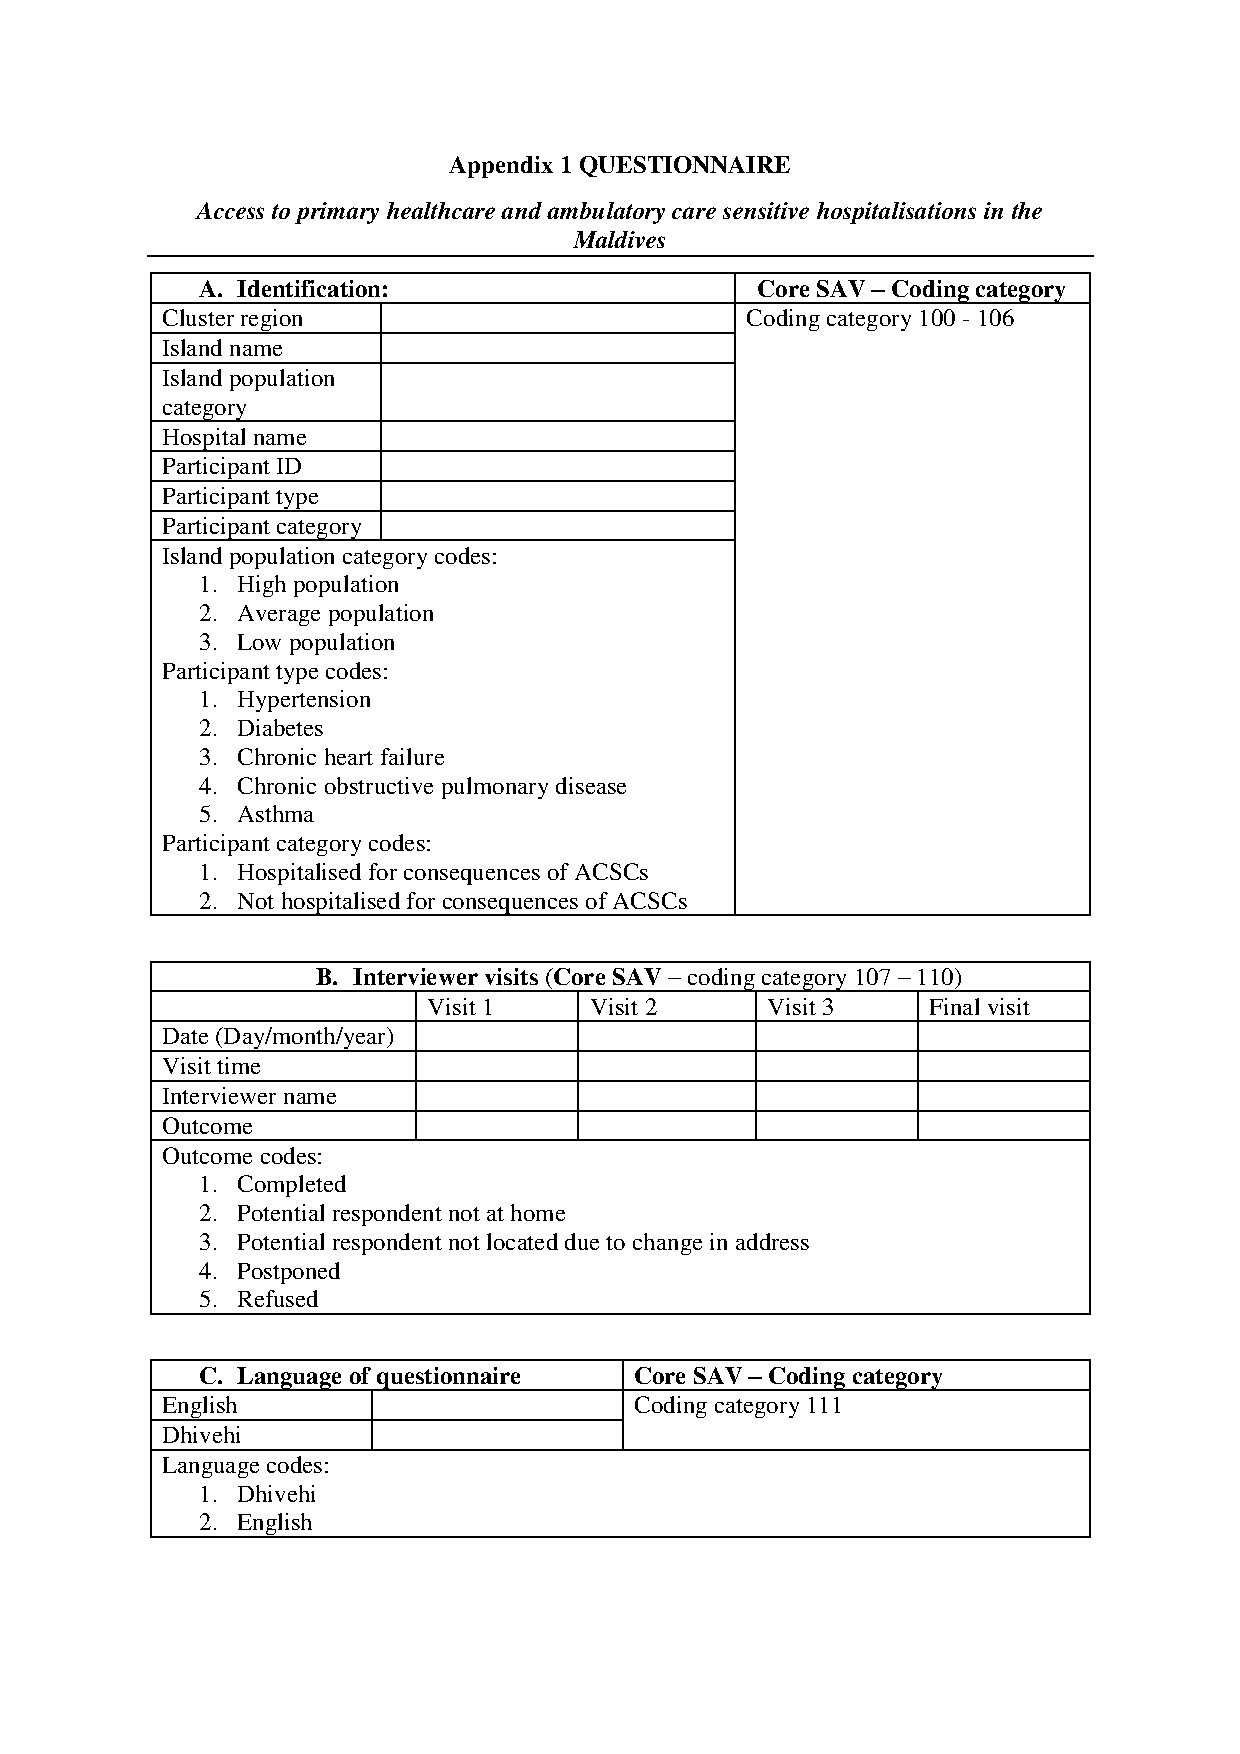
\includepdf[pages=-]{NewTool.pdf}
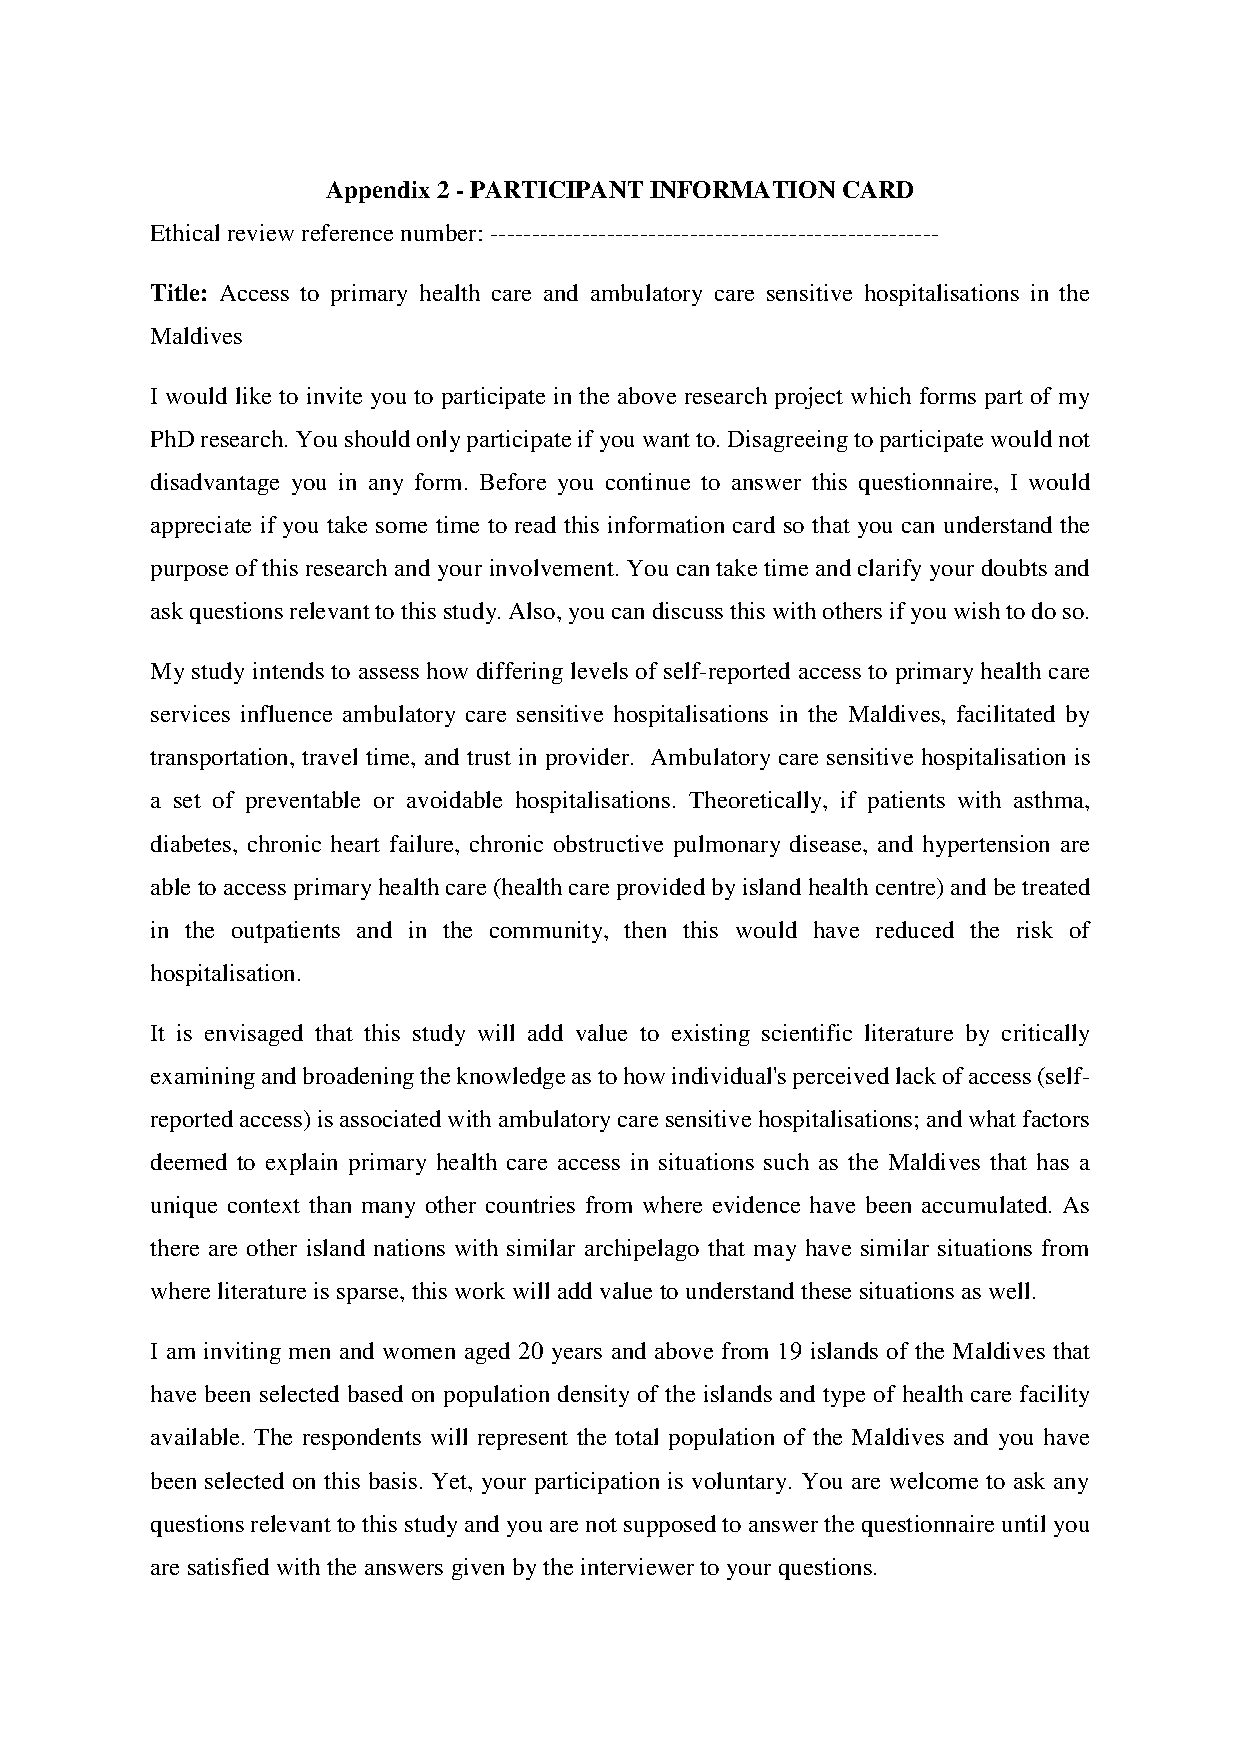
\includepdf[pages=-]{Appendix3.pdf}
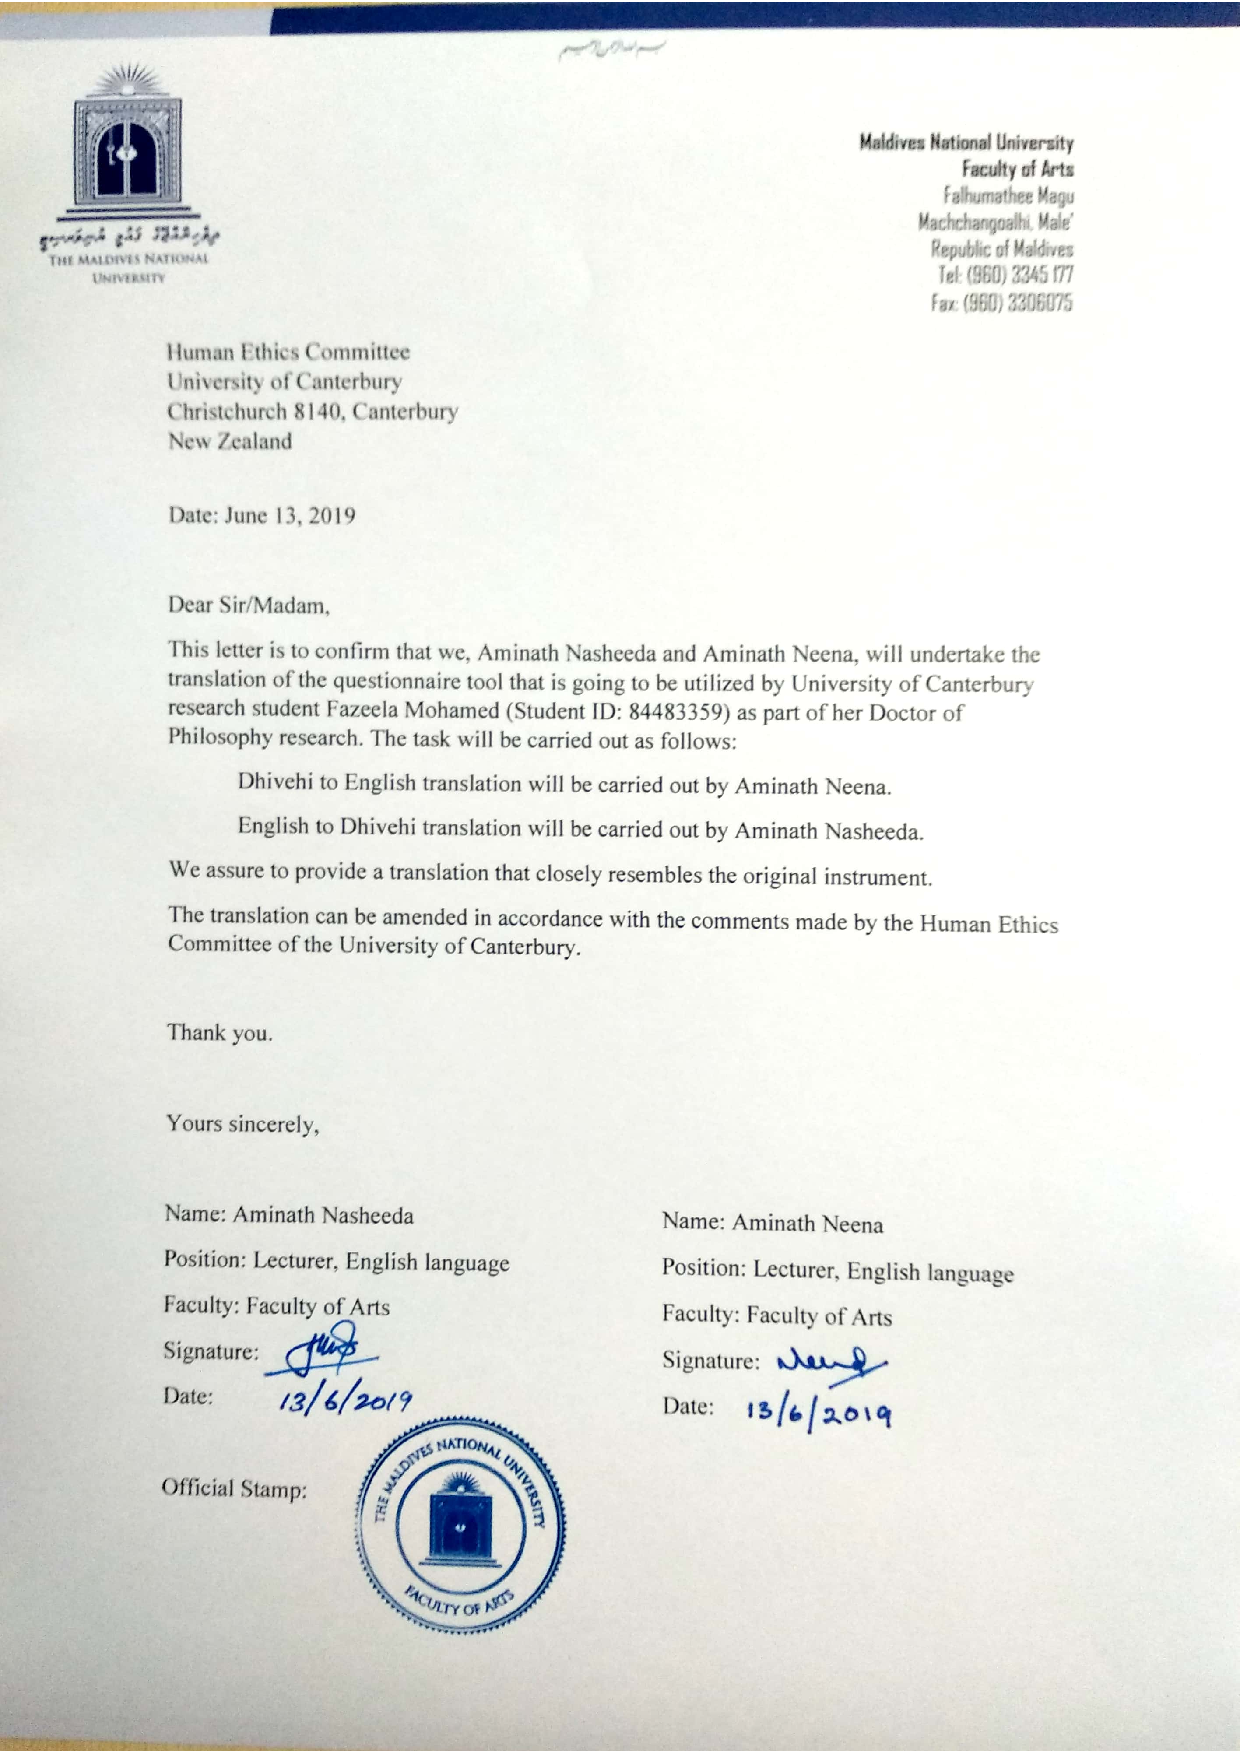
\includepdf[pages=-]{MNULetter.pdf}






































\include{tables}
\newpage
\bibliographystyle{apacite}
\bibliography{ref}
\end{document}

